\documentclass[11pt,a4paper, x11names]{article}\usepackage[]{graphicx}\usepackage[]{color}
% maxwidth is the original width if it is less than linewidth
% otherwise use linewidth (to make sure the graphics do not exceed the margin)
\makeatletter
\def\maxwidth{ %
  \ifdim\Gin@nat@width>\linewidth
    \linewidth
  \else
    \Gin@nat@width
  \fi
}
\makeatother

\definecolor{fgcolor}{rgb}{0, 0, 0}
\makeatletter
\@ifundefined{AddToHook}{}{\AddToHook{package/xcolor/after}{\definecolor{fgcolor}{rgb}{0, 0, 0}}}
\makeatother
\newcommand{\hlnum}[1]{\textcolor[rgb]{0,0,1}{\textbf{#1}}}%
\newcommand{\hlstr}[1]{\textcolor[rgb]{0.639,0.082,0.082}{#1}}%
\newcommand{\hlcom}[1]{\textcolor[rgb]{0.376,0.376,0.376}{#1}}%
\newcommand{\hlopt}[1]{\textcolor[rgb]{0,0,0}{#1}}%
\newcommand{\hlstd}[1]{\textcolor[rgb]{0,0,0}{#1}}%
\newcommand{\hlkwa}[1]{\textcolor[rgb]{0,0,1}{#1}}%
\newcommand{\hlkwb}[1]{\textcolor[rgb]{0,0,1}{#1}}%
\newcommand{\hlkwc}[1]{\textcolor[rgb]{0.169,0.569,0.686}{#1}}%
\newcommand{\hlkwd}[1]{\textcolor[rgb]{0.169,0.569,0.686}{#1}}%
\let\hlipl\hlkwb

\usepackage{framed}
\makeatletter
\newenvironment{kframe}{%
 \def\at@end@of@kframe{}%
 \ifinner\ifhmode%
  \def\at@end@of@kframe{\end{minipage}}%
  \begin{minipage}{\columnwidth}%
 \fi\fi%
 \def\FrameCommand##1{\hskip\@totalleftmargin \hskip-\fboxsep
 \colorbox{shadecolor}{##1}\hskip-\fboxsep
     % There is no \\@totalrightmargin, so:
     \hskip-\linewidth \hskip-\@totalleftmargin \hskip\columnwidth}%
 \MakeFramed {\advance\hsize-\width
   \@totalleftmargin\z@ \linewidth\hsize
   \@setminipage}}%
 {\par\unskip\endMakeFramed%
 \at@end@of@kframe}
\makeatother

\definecolor{shadecolor}{rgb}{.97, .97, .97}
\definecolor{messagecolor}{rgb}{0, 0, 0}
\definecolor{warningcolor}{rgb}{1, 0, 1}
\definecolor{errorcolor}{rgb}{1, 0, 0}
\makeatletter
\@ifundefined{AddToHook}{}{\AddToHook{package/xcolor/after}{
\definecolor{shadecolor}{rgb}{.97, .97, .97}
\definecolor{messagecolor}{rgb}{0, 0, 0}
\definecolor{warningcolor}{rgb}{1, 0, 1}
\definecolor{errorcolor}{rgb}{1, 0, 0}
}}
\makeatother
\newenvironment{knitrout}{}{} % an empty environment to be redefined in TeX

\usepackage{alltt}
\usepackage[utf8]{inputenc}
\usepackage[french]{babel}
\usepackage[left=2cm,right=2cm,top=2cm,bottom=2cm]{geometry}
\usepackage[colorlinks=true,linkcolor=black,anchorcolor=black,citecolor=black,filecolor=black,menucolor=black,runcolor=black,urlcolor=black]{hyperref} 
\usepackage[T1]{fontenc} % Font encoding
\usepackage{graphicx}
\graphicspath{{Images/}}
\usepackage{eso-pic} 
\usepackage{subfig} 
\usepackage{caption} 
\usepackage{tabu}
\usepackage{longtable}
\usepackage{transparent}
\usepackage{amsmath}
\usepackage{amsthm}
\usepackage{bm}
\usepackage{mdframed}
\usepackage[overload]{empheq}  
\usepackage{tabularx}
\usepackage{longtable}
\usepackage{colortbl}
\usepackage{cleveref}
\usepackage[square, numbers, sort&compress]{natbib} 
\bibliographystyle{plain} 
\usepackage{appendix}
\usepackage{enumitem}
\usepackage{amsthm,thmtools,xcolor} 
\usepackage{comment} % Comment part of code
\usepackage{fancyhdr} % Fancy headers and footers
\usepackage{tcolorbox} 
\usepackage{amsmath,amsfonts,amssymb}
\usepackage{pgfplots,tikz}
\usetikzlibrary{matrix}
\usepackage{enumitem}  
\usepackage[normalem]{ulem}
%fonts change 
\usepackage[charter]{mathdesign}
\usepackage{fancybox,framed}
\tcbuselibrary{skins,breakable,xparse}
\usepackage{shadowtext}
\usepackage{titlesec}
\usepackage{setspace}

\usepackage{booktabs}
\usepackage{caption}
\usepackage{float}
\usepackage{titlesec}
\usepackage{capt-of}

%dashed line
\usepackage{array}
\usepackage{arydshln}
\setlength\dashlinedash{0.2pt}
\setlength\dashlinegap{1.5pt}
\setlength\arrayrulewidth{0.3pt}

%Widows & Orphans & Penalties

\widowpenalty500
\clubpenalty500
\clubpenalty=9996
\exhyphenpenalty=50 %for line-breaking at an explicit hyphen
\brokenpenalty=4991
\predisplaypenalty=10000
\postdisplaypenalty=1549
\displaywidowpenalty=1602
\floatingpenalty = 20000
\setstretch{1.5}
\pagestyle{fancy}
\renewcommand{\footrulewidth}{0pt}
\renewcommand{\headrulewidth}{1pt}
\setlist[enumerate,1]{label=\arabic*)}
\setlength{\parindent}{0mm}
\titleformat{\section}
{\normalfont\Large\bfseries}{\thesection .}{1.5mm}{}
\titleformat{\subsection}
{\normalfont\large\bfseries}{\thesubsection}{1.5mm}{}
\titleformat{\subsubsection}
{\normalfont\normalsize\bfseries}{\thesubsubsection}{1.5mm}{}
\titleformat{\paragraph}[runin]
{\normalfont\normalsize\bfseries}{\theparagraph}{1.5mm}{}
\titleformat{\subparagraph}[runin]
{\normalfont\normalsize\bfseries}{\thesubparagraph}{1.5mm}{}

\renewcommand{\d}{\,\mathrm{d}}    

\renewcommand{\title}{Certificat de spécialisation analyste de données massives}
% -> author name and surname
\newcommand{\authora}{Boukary OUEDRAOGO}
\newcommand{\authorb}{Bangaly CAMARA}
\newcommand{\authorc}{Imad EL HAMMA}
% -> MSc course
\newcommand{\course}{STA211}
\newcommand{\advisor}{Mme Niang}
% IF AND ONLY IF you need to modify the co-supervisors you also have to modify the file Configuration_files/title_page.tex (ONLY where it is marked)
\newcommand{\firstcoadvisor}{Name Surname} % insert if any otherwise comment
\newcommand{\secondcoadvisor}{Name Surname} % insert if any otherwise comment
% -> author ID
\newcommand{\ID}{Student ID}
% -> academic year
\newcommand{\YEAR}{2021-2022}
\definecolor{bluePoli}{rgb}{0.87, 0.36, 0.51}
\definecolor{babyblueeyes}{rgb}{0.63, 0.79, 0.95}
\definecolor{blush}{rgb}{0.87, 0.36, 0.51}
\definecolor{bubblegum}{rgb}{0.99, 0.76, 0.8}
\definecolor{charcoal}{rgb}{0.21, 0.27, 0.31}
% Custom theorem environments
\declaretheoremstyle[
  headfont=\color{bluePoli}\normalfont\bfseries,
  bodyfont=\color{black}\normalfont\itshape,
]{colored}

\captionsetup[figure]{labelfont={color=charcoal}} % Set colour of the captions
\captionsetup[table]{labelfont={color=charcoal}} % Set colour of the captions
\captionsetup[algorithm]{labelfont={color=charcoal}} % Set colour of the captions

\theoremstyle{colored}
\newtheorem{theorem}{Theorem}[section]
\newtheorem{proposition}{Proposition}[section]

% Enhances the features of the standard "table" and "tabular" environments.
\newcommand\T{\rule{0pt}{2.6ex}}
\newcommand\B{\rule[-1.2ex]{0pt}{0pt}}

% Algorithm description
\newcounter{algsubstate}
\renewcommand{\thealgsubstate}{\alph{algsubstate}}
\newenvironment{algsubstates}{
  \setcounter{algsubstate}{0}%
  \renewcommand{\STATE}{%
    \stepcounter{algsubstate}%
    \Statex {\small\thealgsubstate:}\space}
}{}

% Custom theorem environment
\newcolumntype{L}[1]{>{\raggedright\let\newline\\\arraybackslash\hspace{0pt}}m{#1}}
  \newcolumntype{C}[1]{>{\centering\let\newline\\\arraybackslash\hspace{0pt}}m{#1}}
    \newcolumntype{R}[1]{>{\raggedleft\let\newline\\\arraybackslash\hspace{0pt}}m{#1}}
      
      % Custom itemize environment
      \setlist[itemize,1]{label=$\bullet$}
      \setlist[itemize,2]{label=$\circ$}
      \setlist[itemize,3]{label=$-$}
      \setlist{nosep}
      
      % Create command for background pic
      \newcommand\BackgroundPic{% Adding background picture
        \put(237,365){
          \parbox[b][\paperheight]{\paperwidth}{%
            \vfill
            \centering
            \transparent{0.4}
            \includegraphics[width=0.44\paperwidth]{raggiera_polimi.eps}%
            \vfill}
        }
      }
      
      % Set indentation
      \setlength\parindent{0pt}
      
      % Custom title commands
      \titleformat{\section}
      {\color{charcoal}\normalfont\Large\bfseries}
      {\color{charcoal}\thesection.}{1em}{}
      \titlespacing*{\section}
      {0pt}{3.3ex}{3.3ex}
      
      \titleformat{\subsection}
      {\color{charcoal}\normalfont\large\bfseries}
      {\color{charcoal}\thesubsection.}{1em}{}
      \titlespacing*{\subsection}
      {0pt}{3.3ex}{3.3ex}
      
      % Custom headers and footers
      \pagestyle{fancy}
      \fancyhf{}
      
      \fancyfoot{}
      \fancyfoot[C]{\thepage} % page
      \renewcommand{\headrulewidth}{0mm} % headrule width
      \renewcommand{\footrulewidth}{0mm} % footrule width
      
      \makeatletter
      \patchcmd{\headrule}{\hrule}{\color{black}\hrule}{}{} % headrule
      \patchcmd{\footrule}{\hrule}{\color{black}\hrule}{}{} % footrule
      \makeatother
\IfFileExists{upquote.sty}{\usepackage{upquote}}{}
\begin{document}


\begin{titlepage}
\thispagestyle{empty}

\begin{tikzpicture}[remember picture,overlay]
\node at (current page.south west)
{\begin{tikzpicture}[remember picture, overlay]
  \shade[bottom color=bubblegum,top color=white] (0,0) rectangle
  (\paperwidth,.7\paperheight);
  \node [color=gray!50,rotate=-20]at (0.35\textwidth,9){\resizebox{7cm}{1.5cm}{$\displaystyle u(x)\approx U_h=\sum_{j=1}^{N}c_j\varphi_j(x)$}};
  \node [color=gray!50,rotate=-5]at (.8\textwidth,5){\resizebox{9cm}{1.5cm}{$ \displaystyle u''(x_i ) \approx\dfrac{1}{h^2}\left[u(x_{ i+1} ) - 2u(x_i ) + u(x_{i-1 } )\right] $}
  };
  \end{tikzpicture}
};

\end{tikzpicture}
\vspace{-1cm}
%-----------------------------------------------------------------------------------
  %  page de garde
%-----------------------------------------------------------------------------------
  \begin{center}

\begin{large}

\includegraphics[scale=0.5]{Images/logocnam.png} \\
\textsc{Certificat de spécialisation analyste de données massives}\\ \bigskip
\textbf{ Entreposage et fouille de données
} \end{large}
\end{center}
\bigskip
\shadowoffset{3pt}
\begin{tcolorbox}[blanker,top=1.2cm,bottom=1.2cm,borderline horizontal={4pt}{0pt}{charcoal},colupper=bluePoli]
\begin{center}
\shadowtext{\resizebox{\textwidth}{1.5cm}{\textbf{Projet de STA211} }}
\end{center}
\end{tcolorbox}


\bigskip

\begin{minipage}{0.4\textwidth}
\large
\emph{Auteurs:}\\
\authora\\[3mm]
\authorb\\[3mm]
\authorc\\[3mm]
\end{minipage}
\hfill
\begin{minipage}{0.4\textwidth}
 \large
\emph{Professeur:}\\
\advisor\\[3mm]
\\[3mm]
\\[3mm]
\end{minipage}\\[2cm] 


\textcolor{charcoal}{\rule{.82\textwidth}{4pt}\hfill {\fontfamily{pzc}\fontsize{.7cm}{0cm}\selectfont \YEAR }}
\end{titlepage}
\begin{abstract}

\end{abstract}
\section{Introduction}





\section{Chargement des données et analyses préliminaires}
Cette partie est consacrée au chargement des données et à la sélection des variables 
liées au ménage. Certaines variables qui sont codées comme des variables numériques mais qui en réalité sont qualitatives seront recordées en variables facteurs.  
\subsection{Chargement des données}


% Analyse univariée
Après le chargement des données, l'étape suivante est l'analyse univariée. 
On peut regarder les statistiques descriptives simples avec la function \textbf{summary} et la fonction \textbf{describe}.

\begin{knitrout}
\definecolor{shadecolor}{rgb}{1, 1, 1}\color{fgcolor}\begin{kframe}
\begin{verbatim}
##  Sexe      Diplome_Max  Type_Prof Occupation Source_ppale_Res Structure_menage
##  1: 549   4      :454   1: 36     1:777      1:845            1: 398          
##  2:1018   8      :175   2: 70     2: 80      2: 87            2: 103          
##           1      :171   3:435     3: 50      3:493            3:1053          
##           9      :168   4:391     4:541      4: 71            4:  13          
##           6      :157   5:297     5: 45      5: 71                            
##           5      :137   6:316     6: 74                                       
##           (Other):305   7: 22                                                 
##       Age           Revenus     TYPEMEN Nb_Enfants_sup_10 Nb_Enfants_inf_10
##  Min.   :18.00   Min.   : 535   1:190   Min.   :0.0000    Min.   :0.0000   
##  1st Qu.:41.00   1st Qu.:1799   2:144   1st Qu.:0.0000    1st Qu.:0.0000   
##  Median :52.00   Median :2349   3: 75   Median :0.0000    Median :0.0000   
##  Mean   :51.87   Mean   :2573   4:301   Mean   :0.4359    Mean   :0.3165   
##  3rd Qu.:61.50   3rd Qu.:2899   5:114   3rd Qu.:1.0000    3rd Qu.:0.0000   
##  Max.   :89.00   Max.   :7600   6:228   Max.   :3.0000    Max.   :3.0000   
##                                 7:515
## Description of .
## 
##  Numeric 
##                      mean median min  max        var      sd
## Age                 51.87     52  18   89     209.91   14.49
## Revenus           2573.20   2349 535 7600 1967644.23 1402.73
## Nb_Enfants_sup_10    0.44      0   0    3       0.67    0.82
## Nb_Enfants_inf_10    0.32      0   0    3       0.48    0.70
## 
##  Factor 
##          
## Sexe            2      1
##   Count   1018.00 549.00
##   Percent   64.96  35.04
## Mode 2 
##            
## Diplome_Max      4      8      1      9      6      5      7      3     2
##     Count   454.00 175.00 171.00 168.00 157.00 137.00 132.00 117.00 56.00
##     Percent  28.97  11.17  10.91  10.72  10.02   8.74   8.42   7.47  3.57
## Mode 4 
##          
## Type_Prof      3      4      6      5     2    1    7
##   Count   435.00 391.00 316.00 297.00 70.00 36.0 22.0
##   Percent  27.76  24.95  20.17  18.95  4.47  2.3  1.4
## Mode 3 
##           
## Occupation      1      4     2     6     3     5
##    Count   777.00 541.00 80.00 74.00 50.00 45.00
##    Percent  49.59  34.52  5.11  4.72  3.19  2.87
## Mode 1 
##                 
## Source_ppale_Res      1      3     2     4     5
##          Count   845.00 493.00 87.00 71.00 71.00
##          Percent  53.92  31.46  5.55  4.53  4.53
## Mode 1 
##                 
## Structure_menage      3     1      2     4
##          Count   1053.0 398.0 103.00 13.00
##          Percent   67.2  25.4   6.57  0.83
## Mode 3 
##          
## TYPEMEN        7      4      6      1      2      5     3
##   Count   515.00 301.00 228.00 190.00 144.00 114.00 75.00
##   Percent  32.87  19.21  14.55  12.13   9.19   7.28  4.79
## Mode 7
\end{verbatim}
\end{kframe}
\end{knitrout}

%-------------------------------------------------------------------------------
%  SECTION 1: Variables quantitatives
%-------------------------------------------------------------------------------
\subsection{Analyse descriptive des variables quantitatives }
\subsubsection{Analyse univarié}

\begin{table*}[!h] \centering
%\ra{1.3}
\begin{small}
\begin{tabular}{@{}lrrrrrr@{}}\toprule
\textbf{Variables}& \textbf{Moyenne} & \textbf{Médiane}& \textbf{Min} & \textbf{Maximum} & \textbf{Variance} & \textbf{Ecart-type} \\ \midrule
\textbf{Age}          & 51.87 &  52 & 18 & 89 & 209.91 & 14.49\ \\ \hdashline
\textbf{Revenus}      & 2~573.20 & 2~349 & 535&7~600 & 1~967~644.23&1~402.73   \\ \hdashline
\textbf{Nombre d'enfants dont âge > 10 ans} &  0.44 & 0 & 0 & 3 & 0.67 & 0.82  \\  \hdashline
\textbf{Nombre d'enfants dont âge <= 10 ans} &  0.32 & 0 & 0 & 3 & 0.48 & 0.70 \\  
\bottomrule
\end{tabular}
\end{small}
\caption{Statistiques descriptives des variables quantitatives}
\end{table*}


%-------------------------------------------------------------------------------
%   SECTION 2: Variables qualitatives
%-------------------------------------------------------------------------------

\subsubsection{Analyse bivariée: Etudes des liaisons entre les différentes variables quantitatives}

\begin{framed}
\begin{knitrout}
\definecolor{shadecolor}{rgb}{1, 1, 1}\color{fgcolor}
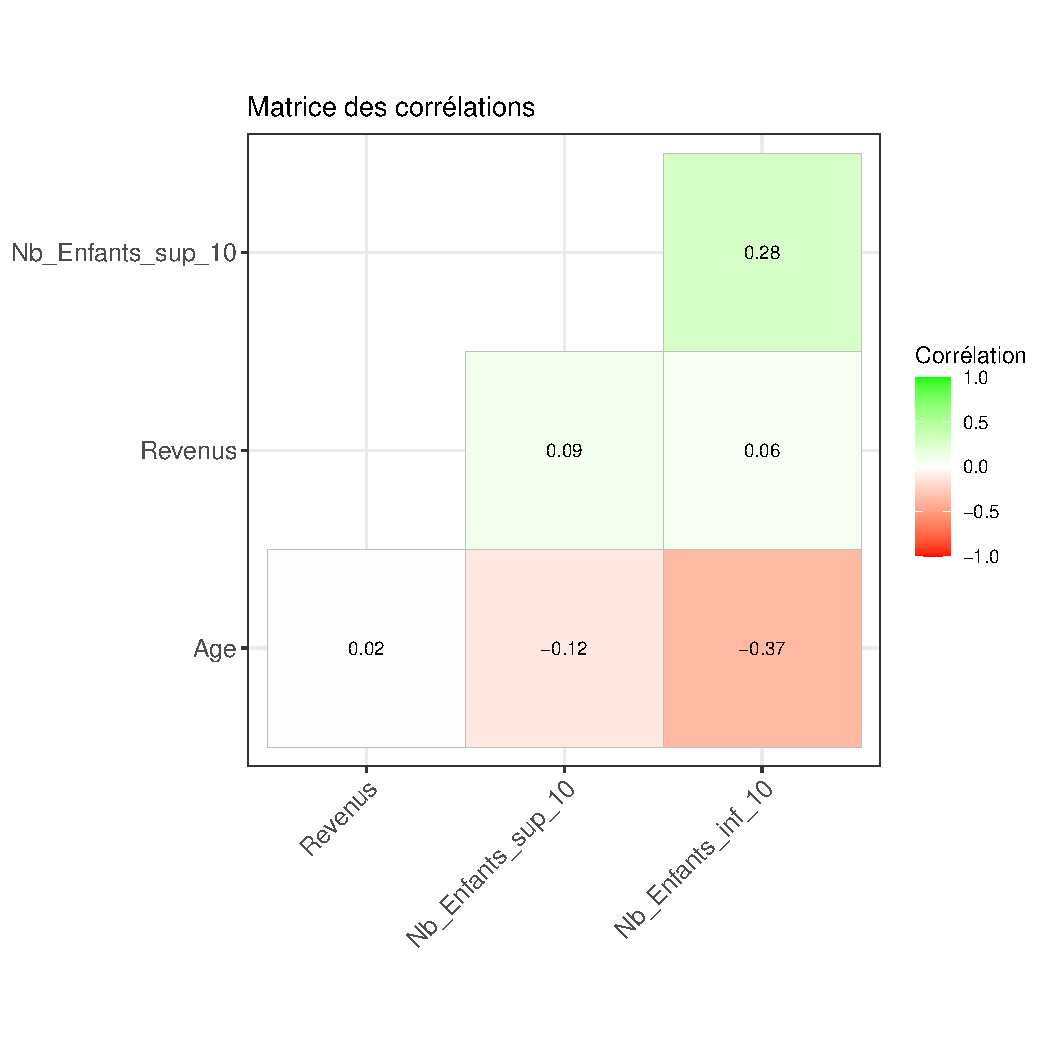
\includegraphics[width=\maxwidth]{figure/unnamed-chunk-5-1} 
\end{knitrout}
\end{framed}




\begin{mdframed}[linecolor=blue]
\begin{knitrout}
\definecolor{shadecolor}{rgb}{1, 1, 1}\color{fgcolor}
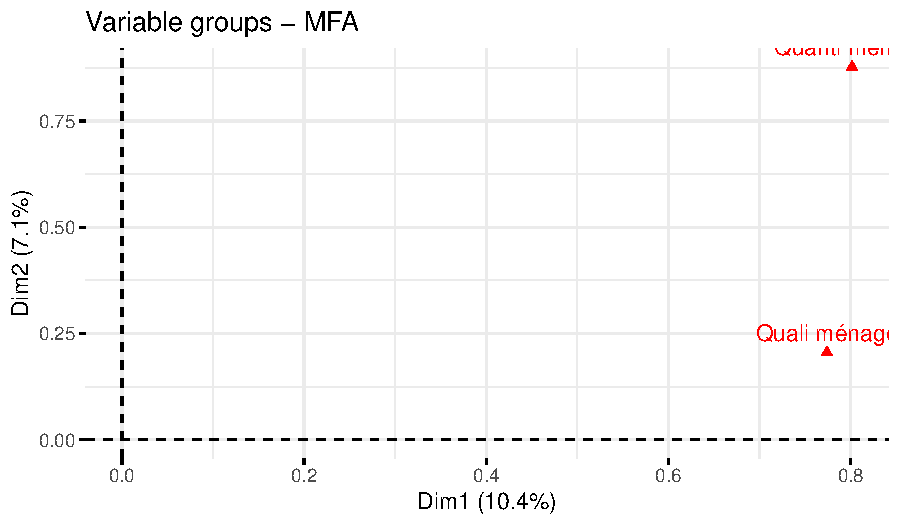
\includegraphics[width=\maxwidth]{figure/unnamed-chunk-8-1} 
\end{knitrout}
\end{mdframed}

\begin{knitrout}
\definecolor{shadecolor}{rgb}{1, 1, 1}\color{fgcolor}
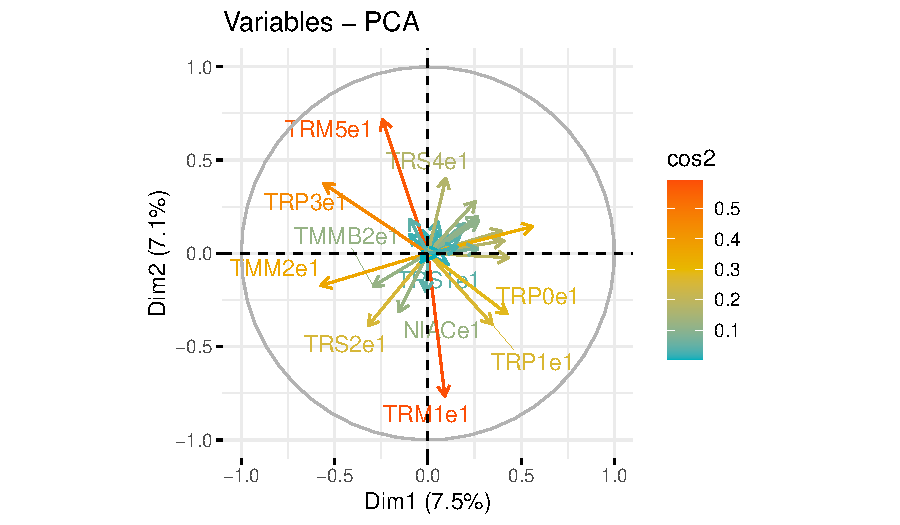
\includegraphics[width=\maxwidth]{figure/unnamed-chunk-9-1} 

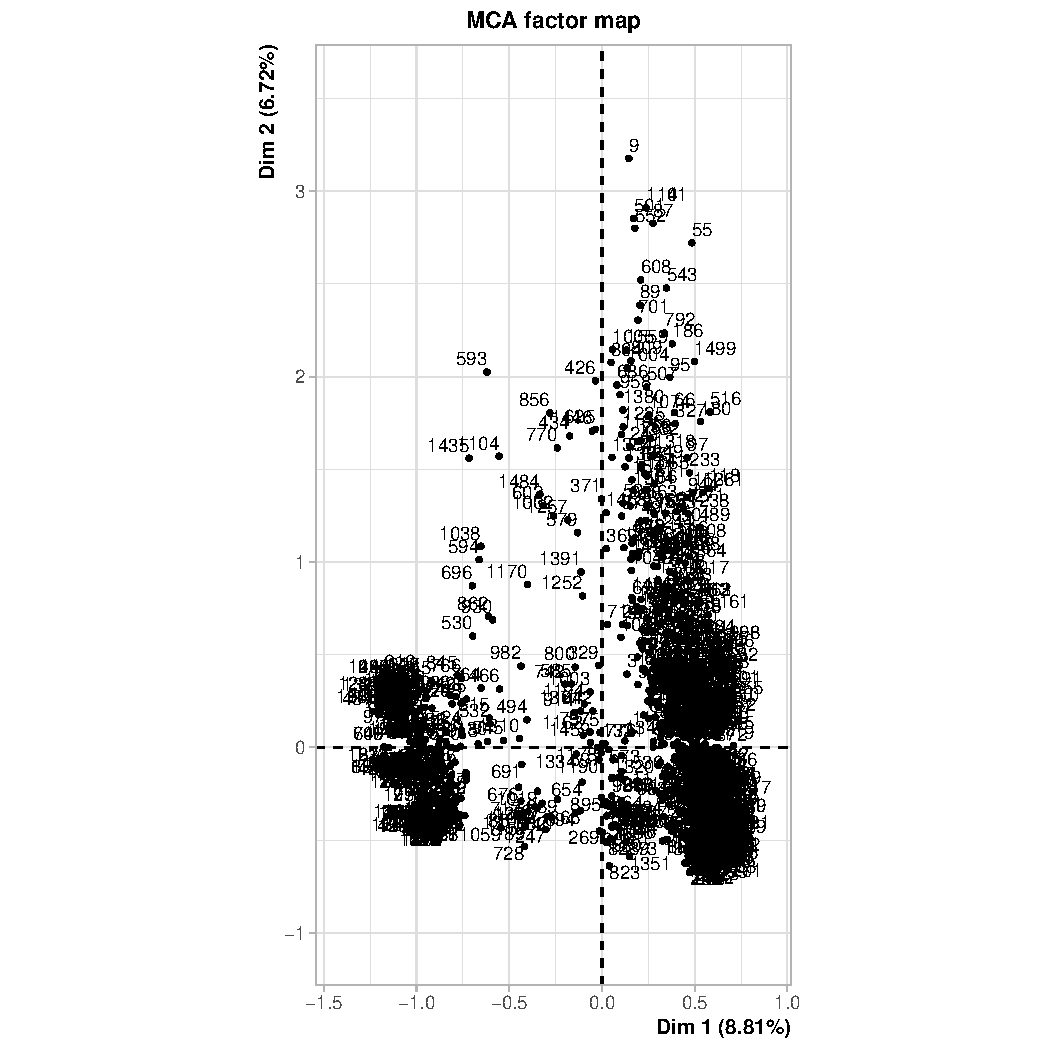
\includegraphics[width=\maxwidth]{figure/unnamed-chunk-9-2} 

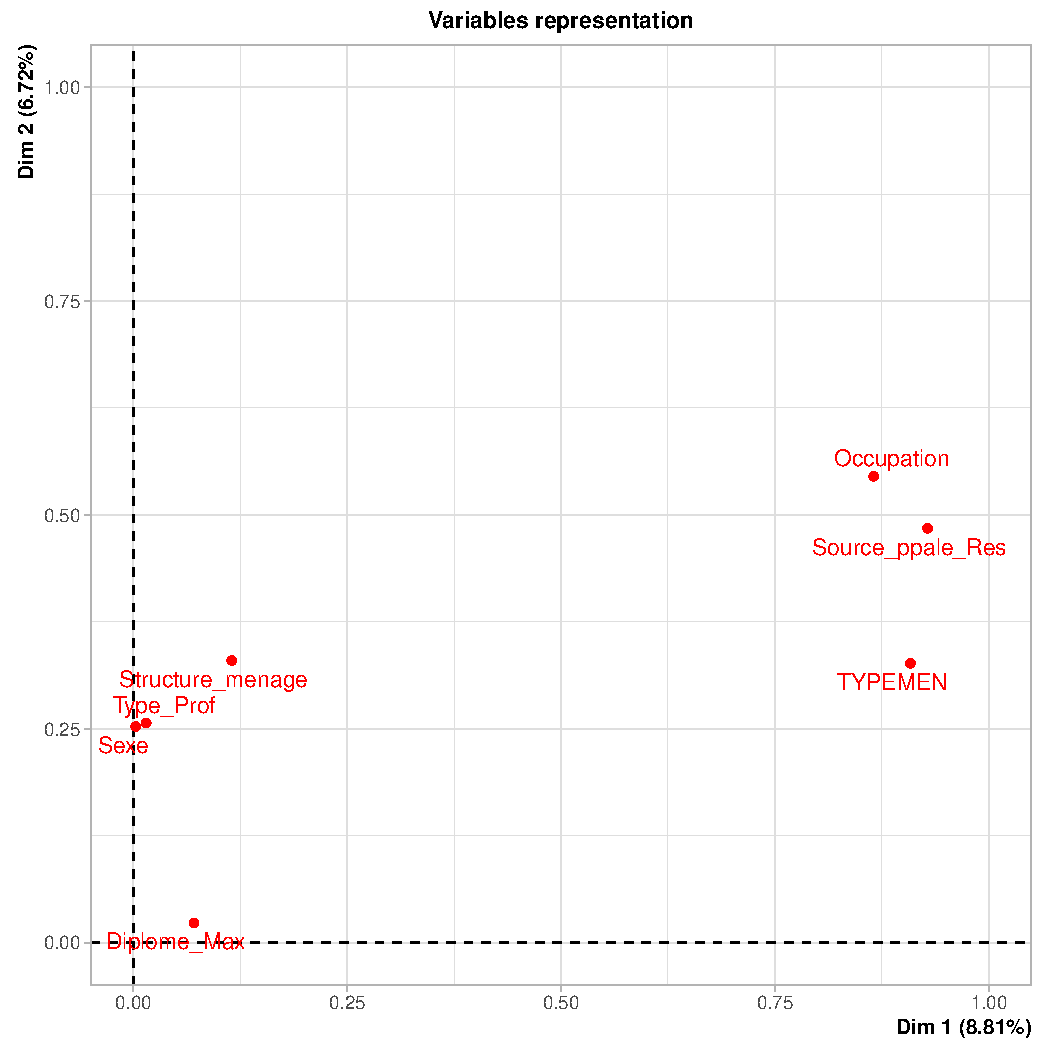
\includegraphics[width=\maxwidth]{figure/unnamed-chunk-9-3} 

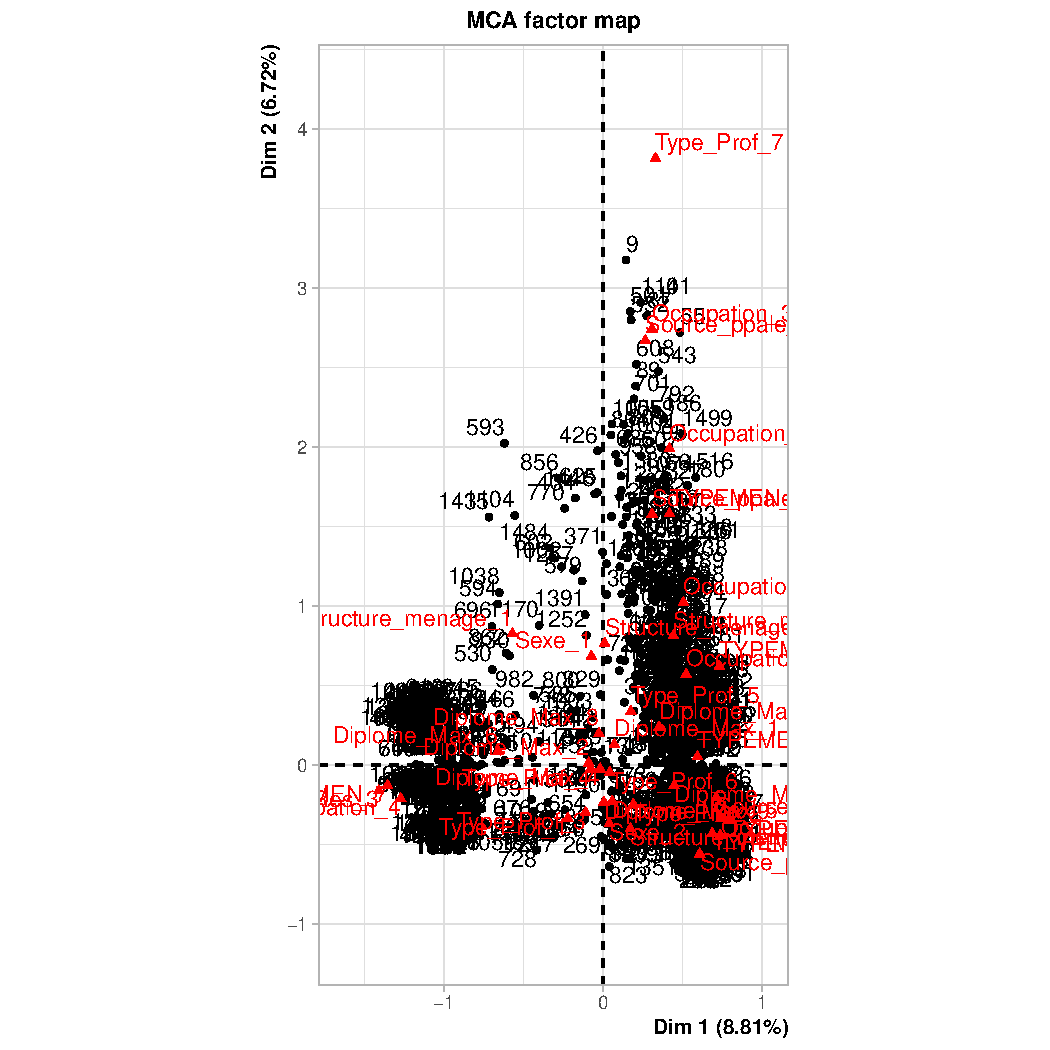
\includegraphics[width=\maxwidth]{figure/unnamed-chunk-9-4} 
\end{knitrout}

%  Khi2
\begin{knitrout}
\definecolor{shadecolor}{rgb}{1, 1, 1}\color{fgcolor}\begin{kframe}
\begin{verbatim}
## [1] "----------------Sexe  CONTRE  Diplome_Max------------------"
## 
## 	Pearson's Chi-squared test
## 
## data:  data_cat_plots[, i] and data_cat_plots[, j]
## X-squared = 20.566, df = 8, p-value = 0.008393
## 
## [1] "----------------Sexe  CONTRE  Type_Prof------------------"
## 
## 	Pearson's Chi-squared test
## 
## data:  data_cat_plots[, i] and data_cat_plots[, j]
## X-squared = 41.855, df = 6, p-value = 1.964e-07
## 
## [1] "----------------Sexe  CONTRE  Occupation------------------"
## 
## 	Pearson's Chi-squared test
## 
## data:  data_cat_plots[, i] and data_cat_plots[, j]
## X-squared = 112.29, df = 5, p-value < 2.2e-16
## 
## [1] "----------------Sexe  CONTRE  Source_ppale_Res------------------"
## 
## 	Pearson's Chi-squared test
## 
## data:  data_cat_plots[, i] and data_cat_plots[, j]
## X-squared = 28.434, df = 4, p-value = 1.019e-05
## 
## [1] "----------------Sexe  CONTRE  Structure_menage------------------"
## 
## 	Pearson's Chi-squared test
## 
## data:  data_cat_plots[, i] and data_cat_plots[, j]
## X-squared = 191.39, df = 3, p-value < 2.2e-16
## 
## [1] "----------------Sexe  CONTRE  TYPEMEN------------------"
## 
## 	Pearson's Chi-squared test
## 
## data:  data_cat_plots[, i] and data_cat_plots[, j]
## X-squared = 146.96, df = 6, p-value < 2.2e-16
## 
## [1] "----------------Diplome_Max  CONTRE  Sexe------------------"
## 
## 	Pearson's Chi-squared test
## 
## data:  data_cat_plots[, i] and data_cat_plots[, j]
## X-squared = 20.566, df = 8, p-value = 0.008393
## 
## [1] "----------------Diplome_Max  CONTRE  Type_Prof------------------"
## 
## 	Pearson's Chi-squared test
## 
## data:  data_cat_plots[, i] and data_cat_plots[, j]
## X-squared = 193.54, df = 48, p-value < 2.2e-16
## 
## [1] "----------------Diplome_Max  CONTRE  Occupation------------------"
## 
## 	Pearson's Chi-squared test
## 
## data:  data_cat_plots[, i] and data_cat_plots[, j]
## X-squared = 83.567, df = 40, p-value = 6.568e-05
## 
## [1] "----------------Diplome_Max  CONTRE  Source_ppale_Res------------------"
## 
## 	Pearson's Chi-squared test
## 
## data:  data_cat_plots[, i] and data_cat_plots[, j]
## X-squared = 74.595, df = 32, p-value = 2.969e-05
## 
## [1] "----------------Diplome_Max  CONTRE  Structure_menage------------------"
## 
## 	Pearson's Chi-squared test
## 
## data:  data_cat_plots[, i] and data_cat_plots[, j]
## X-squared = 26.415, df = 24, p-value = 0.3324
## 
## [1] "----------------Diplome_Max  CONTRE  TYPEMEN------------------"
## 
## 	Pearson's Chi-squared test
## 
## data:  data_cat_plots[, i] and data_cat_plots[, j]
## X-squared = 95.833, df = 48, p-value = 4.999e-05
## 
## [1] "----------------Type_Prof  CONTRE  Sexe------------------"
## 
## 	Pearson's Chi-squared test
## 
## data:  data_cat_plots[, i] and data_cat_plots[, j]
## X-squared = 41.855, df = 6, p-value = 1.964e-07
## 
## [1] "----------------Type_Prof  CONTRE  Diplome_Max------------------"
## 
## 	Pearson's Chi-squared test
## 
## data:  data_cat_plots[, i] and data_cat_plots[, j]
## X-squared = 193.54, df = 48, p-value < 2.2e-16
## 
## [1] "----------------Type_Prof  CONTRE  Occupation------------------"
## 
## 	Pearson's Chi-squared test
## 
## data:  data_cat_plots[, i] and data_cat_plots[, j]
## X-squared = 440.03, df = 30, p-value < 2.2e-16
## 
## [1] "----------------Type_Prof  CONTRE  Source_ppale_Res------------------"
## 
## 	Pearson's Chi-squared test
## 
## data:  data_cat_plots[, i] and data_cat_plots[, j]
## X-squared = 208.64, df = 24, p-value < 2.2e-16
## 
## [1] "----------------Type_Prof  CONTRE  Structure_menage------------------"
## 
## 	Pearson's Chi-squared test
## 
## data:  data_cat_plots[, i] and data_cat_plots[, j]
## X-squared = 43.018, df = 18, p-value = 0.0007957
## 
## [1] "----------------Type_Prof  CONTRE  TYPEMEN------------------"
## 
## 	Pearson's Chi-squared test
## 
## data:  data_cat_plots[, i] and data_cat_plots[, j]
## X-squared = 125.82, df = 36, p-value = 6.912e-12
## 
## [1] "----------------Occupation  CONTRE  Sexe------------------"
## 
## 	Pearson's Chi-squared test
## 
## data:  data_cat_plots[, i] and data_cat_plots[, j]
## X-squared = 112.29, df = 5, p-value < 2.2e-16
## 
## [1] "----------------Occupation  CONTRE  Diplome_Max------------------"
## 
## 	Pearson's Chi-squared test
## 
## data:  data_cat_plots[, i] and data_cat_plots[, j]
## X-squared = 83.567, df = 40, p-value = 6.568e-05
## 
## [1] "----------------Occupation  CONTRE  Type_Prof------------------"
## 
## 	Pearson's Chi-squared test
## 
## data:  data_cat_plots[, i] and data_cat_plots[, j]
## X-squared = 440.03, df = 30, p-value < 2.2e-16
## 
## [1] "----------------Occupation  CONTRE  Source_ppale_Res------------------"
## 
## 	Pearson's Chi-squared test
## 
## data:  data_cat_plots[, i] and data_cat_plots[, j]
## X-squared = 1989.8, df = 20, p-value < 2.2e-16
## 
## [1] "----------------Occupation  CONTRE  Structure_menage------------------"
## 
## 	Pearson's Chi-squared test
## 
## data:  data_cat_plots[, i] and data_cat_plots[, j]
## X-squared = 104.78, df = 15, p-value = 1.61e-15
## 
## [1] "----------------Occupation  CONTRE  TYPEMEN------------------"
## 
## 	Pearson's Chi-squared test
## 
## data:  data_cat_plots[, i] and data_cat_plots[, j]
## X-squared = 1263.4, df = 30, p-value < 2.2e-16
## 
## [1] "----------------Source_ppale_Res  CONTRE  Sexe------------------"
## 
## 	Pearson's Chi-squared test
## 
## data:  data_cat_plots[, i] and data_cat_plots[, j]
## X-squared = 28.434, df = 4, p-value = 1.019e-05
## 
## [1] "----------------Source_ppale_Res  CONTRE  Diplome_Max------------------"
## 
## 	Pearson's Chi-squared test
## 
## data:  data_cat_plots[, i] and data_cat_plots[, j]
## X-squared = 74.595, df = 32, p-value = 2.969e-05
## 
## [1] "----------------Source_ppale_Res  CONTRE  Type_Prof------------------"
## 
## 	Pearson's Chi-squared test
## 
## data:  data_cat_plots[, i] and data_cat_plots[, j]
## X-squared = 208.64, df = 24, p-value < 2.2e-16
## 
## [1] "----------------Source_ppale_Res  CONTRE  Occupation------------------"
## 
## 	Pearson's Chi-squared test
## 
## data:  data_cat_plots[, i] and data_cat_plots[, j]
## X-squared = 1989.8, df = 20, p-value < 2.2e-16
## 
## [1] "----------------Source_ppale_Res  CONTRE  Structure_menage------------------"
## 
## 	Pearson's Chi-squared test
## 
## data:  data_cat_plots[, i] and data_cat_plots[, j]
## X-squared = 163.62, df = 12, p-value < 2.2e-16
## 
## [1] "----------------Source_ppale_Res  CONTRE  TYPEMEN------------------"
## 
## 	Pearson's Chi-squared test
## 
## data:  data_cat_plots[, i] and data_cat_plots[, j]
## X-squared = 1420.4, df = 24, p-value < 2.2e-16
## 
## [1] "----------------Structure_menage  CONTRE  Sexe------------------"
## 
## 	Pearson's Chi-squared test
## 
## data:  data_cat_plots[, i] and data_cat_plots[, j]
## X-squared = 191.39, df = 3, p-value < 2.2e-16
## 
## [1] "----------------Structure_menage  CONTRE  Diplome_Max------------------"
## 
## 	Pearson's Chi-squared test
## 
## data:  data_cat_plots[, i] and data_cat_plots[, j]
## X-squared = 26.415, df = 24, p-value = 0.3324
## 
## [1] "----------------Structure_menage  CONTRE  Type_Prof------------------"
## 
## 	Pearson's Chi-squared test
## 
## data:  data_cat_plots[, i] and data_cat_plots[, j]
## X-squared = 43.018, df = 18, p-value = 0.0007957
## 
## [1] "----------------Structure_menage  CONTRE  Occupation------------------"
## 
## 	Pearson's Chi-squared test
## 
## data:  data_cat_plots[, i] and data_cat_plots[, j]
## X-squared = 104.78, df = 15, p-value = 1.61e-15
## 
## [1] "----------------Structure_menage  CONTRE  Source_ppale_Res------------------"
## 
## 	Pearson's Chi-squared test
## 
## data:  data_cat_plots[, i] and data_cat_plots[, j]
## X-squared = 163.62, df = 12, p-value < 2.2e-16
## 
## [1] "----------------Structure_menage  CONTRE  TYPEMEN------------------"
## 
## 	Pearson's Chi-squared test
## 
## data:  data_cat_plots[, i] and data_cat_plots[, j]
## X-squared = 502.74, df = 18, p-value < 2.2e-16
## 
## [1] "----------------TYPEMEN  CONTRE  Sexe------------------"
## 
## 	Pearson's Chi-squared test
## 
## data:  data_cat_plots[, i] and data_cat_plots[, j]
## X-squared = 146.96, df = 6, p-value < 2.2e-16
## 
## [1] "----------------TYPEMEN  CONTRE  Diplome_Max------------------"
## 
## 	Pearson's Chi-squared test
## 
## data:  data_cat_plots[, i] and data_cat_plots[, j]
## X-squared = 95.833, df = 48, p-value = 4.999e-05
## 
## [1] "----------------TYPEMEN  CONTRE  Type_Prof------------------"
## 
## 	Pearson's Chi-squared test
## 
## data:  data_cat_plots[, i] and data_cat_plots[, j]
## X-squared = 125.82, df = 36, p-value = 6.912e-12
## 
## [1] "----------------TYPEMEN  CONTRE  Occupation------------------"
## 
## 	Pearson's Chi-squared test
## 
## data:  data_cat_plots[, i] and data_cat_plots[, j]
## X-squared = 1263.4, df = 30, p-value < 2.2e-16
## 
## [1] "----------------TYPEMEN  CONTRE  Source_ppale_Res------------------"
## 
## 	Pearson's Chi-squared test
## 
## data:  data_cat_plots[, i] and data_cat_plots[, j]
## X-squared = 1420.4, df = 24, p-value < 2.2e-16
## 
## [1] "----------------TYPEMEN  CONTRE  Structure_menage------------------"
## 
## 	Pearson's Chi-squared test
## 
## data:  data_cat_plots[, i] and data_cat_plots[, j]
## X-squared = 502.74, df = 18, p-value < 2.2e-16
\end{verbatim}
\end{kframe}
\end{knitrout}


%  v cramer
\begin{knitrout}
\definecolor{shadecolor}{rgb}{1, 1, 1}\color{fgcolor}\begin{kframe}
\begin{verbatim}
## [1] "----------------Sexe  CONTRE  Diplome_Max------------------"
##                     X^2 df  P(> X^2)
## Likelihood Ratio 20.349  8 0.0090948
## Pearson          20.566  8 0.0083931
## 
## Phi-Coefficient   : NA 
## Contingency Coeff.: 0.114 
## Cramer's V        : 0.115 
## [1] "----------------Sexe  CONTRE  Type_Prof------------------"
##                     X^2 df   P(> X^2)
## Likelihood Ratio 40.765  6 3.2213e-07
## Pearson          41.855  6 1.9637e-07
## 
## Phi-Coefficient   : NA 
## Contingency Coeff.: 0.161 
## Cramer's V        : 0.163 
## [1] "----------------Sexe  CONTRE  Occupation------------------"
##                     X^2 df P(> X^2)
## Likelihood Ratio 114.46  5        0
## Pearson          112.29  5        0
## 
## Phi-Coefficient   : NA 
## Contingency Coeff.: 0.259 
## Cramer's V        : 0.268 
## [1] "----------------Sexe  CONTRE  Source_ppale_Res------------------"
##                     X^2 df   P(> X^2)
## Likelihood Ratio 27.358  4 1.6825e-05
## Pearson          28.434  4 1.0187e-05
## 
## Phi-Coefficient   : NA 
## Contingency Coeff.: 0.133 
## Cramer's V        : 0.135 
## [1] "----------------Sexe  CONTRE  Structure_menage------------------"
##                     X^2 df P(> X^2)
## Likelihood Ratio 187.89  3        0
## Pearson          191.39  3        0
## 
## Phi-Coefficient   : NA 
## Contingency Coeff.: 0.33 
## Cramer's V        : 0.349 
## [1] "----------------Sexe  CONTRE  TYPEMEN------------------"
##                     X^2 df P(> X^2)
## Likelihood Ratio 145.00  6        0
## Pearson          146.96  6        0
## 
## Phi-Coefficient   : NA 
## Contingency Coeff.: 0.293 
## Cramer's V        : 0.306 
## [1] "----------------Diplome_Max  CONTRE  Sexe------------------"
##                     X^2 df  P(> X^2)
## Likelihood Ratio 20.349  8 0.0090948
## Pearson          20.566  8 0.0083931
## 
## Phi-Coefficient   : NA 
## Contingency Coeff.: 0.114 
## Cramer's V        : 0.115 
## [1] "----------------Diplome_Max  CONTRE  Type_Prof------------------"
##                     X^2 df P(> X^2)
## Likelihood Ratio 189.51 48        0
## Pearson          193.54 48        0
## 
## Phi-Coefficient   : NA 
## Contingency Coeff.: 0.332 
## Cramer's V        : 0.143 
## [1] "----------------Diplome_Max  CONTRE  Occupation------------------"
##                     X^2 df   P(> X^2)
## Likelihood Ratio 84.207 40 5.4822e-05
## Pearson          83.567 40 6.5676e-05
## 
## Phi-Coefficient   : NA 
## Contingency Coeff.: 0.225 
## Cramer's V        : 0.103 
## [1] "----------------Diplome_Max  CONTRE  Source_ppale_Res------------------"
##                     X^2 df   P(> X^2)
## Likelihood Ratio 76.358 32 1.7224e-05
## Pearson          74.595 32 2.9694e-05
## 
## Phi-Coefficient   : NA 
## Contingency Coeff.: 0.213 
## Cramer's V        : 0.109 
## [1] "----------------Diplome_Max  CONTRE  Structure_menage------------------"
##                     X^2 df P(> X^2)
## Likelihood Ratio 27.771 24  0.26983
## Pearson          26.415 24  0.33245
## 
## Phi-Coefficient   : NA 
## Contingency Coeff.: 0.129 
## Cramer's V        : 0.075 
## [1] "----------------Diplome_Max  CONTRE  TYPEMEN------------------"
##                     X^2 df   P(> X^2)
## Likelihood Ratio 96.543 48 4.1295e-05
## Pearson          95.833 48 4.9992e-05
## 
## Phi-Coefficient   : NA 
## Contingency Coeff.: 0.24 
## Cramer's V        : 0.101 
## [1] "----------------Type_Prof  CONTRE  Sexe------------------"
##                     X^2 df   P(> X^2)
## Likelihood Ratio 40.765  6 3.2213e-07
## Pearson          41.855  6 1.9637e-07
## 
## Phi-Coefficient   : NA 
## Contingency Coeff.: 0.161 
## Cramer's V        : 0.163 
## [1] "----------------Type_Prof  CONTRE  Diplome_Max------------------"
##                     X^2 df P(> X^2)
## Likelihood Ratio 189.51 48        0
## Pearson          193.54 48        0
## 
## Phi-Coefficient   : NA 
## Contingency Coeff.: 0.332 
## Cramer's V        : 0.143 
## [1] "----------------Type_Prof  CONTRE  Occupation------------------"
##                     X^2 df P(> X^2)
## Likelihood Ratio 291.71 30        0
## Pearson          440.03 30        0
## 
## Phi-Coefficient   : NA 
## Contingency Coeff.: 0.468 
## Cramer's V        : 0.237 
## [1] "----------------Type_Prof  CONTRE  Source_ppale_Res------------------"
##                     X^2 df P(> X^2)
## Likelihood Ratio 156.66 24        0
## Pearson          208.64 24        0
## 
## Phi-Coefficient   : NA 
## Contingency Coeff.: 0.343 
## Cramer's V        : 0.182 
## [1] "----------------Type_Prof  CONTRE  Structure_menage------------------"
##                     X^2 df   P(> X^2)
## Likelihood Ratio 41.670 18 0.00122949
## Pearson          43.018 18 0.00079568
## 
## Phi-Coefficient   : NA 
## Contingency Coeff.: 0.163 
## Cramer's V        : 0.096 
## [1] "----------------Type_Prof  CONTRE  TYPEMEN------------------"
##                     X^2 df   P(> X^2)
## Likelihood Ratio 121.03 36 3.9728e-11
## Pearson          125.82 36 6.9120e-12
## 
## Phi-Coefficient   : NA 
## Contingency Coeff.: 0.273 
## Cramer's V        : 0.116 
## [1] "----------------Occupation  CONTRE  Sexe------------------"
##                     X^2 df P(> X^2)
## Likelihood Ratio 114.46  5        0
## Pearson          112.29  5        0
## 
## Phi-Coefficient   : NA 
## Contingency Coeff.: 0.259 
## Cramer's V        : 0.268 
## [1] "----------------Occupation  CONTRE  Diplome_Max------------------"
##                     X^2 df   P(> X^2)
## Likelihood Ratio 84.207 40 5.4822e-05
## Pearson          83.567 40 6.5676e-05
## 
## Phi-Coefficient   : NA 
## Contingency Coeff.: 0.225 
## Cramer's V        : 0.103 
## [1] "----------------Occupation  CONTRE  Type_Prof------------------"
##                     X^2 df P(> X^2)
## Likelihood Ratio 291.71 30        0
## Pearson          440.03 30        0
## 
## Phi-Coefficient   : NA 
## Contingency Coeff.: 0.468 
## Cramer's V        : 0.237 
## [1] "----------------Occupation  CONTRE  Source_ppale_Res------------------"
##                     X^2 df P(> X^2)
## Likelihood Ratio 1811.8 20        0
## Pearson          1989.8 20        0
## 
## Phi-Coefficient   : NA 
## Contingency Coeff.: 0.748 
## Cramer's V        : 0.563 
## [1] "----------------Occupation  CONTRE  Structure_menage------------------"
##                     X^2 df   P(> X^2)
## Likelihood Ratio 100.46 15 1.0658e-14
## Pearson          104.78 15 1.6653e-15
## 
## Phi-Coefficient   : NA 
## Contingency Coeff.: 0.25 
## Cramer's V        : 0.149 
## [1] "----------------Occupation  CONTRE  TYPEMEN------------------"
##                     X^2 df P(> X^2)
## Likelihood Ratio 1376.8 30        0
## Pearson          1263.4 30        0
## 
## Phi-Coefficient   : NA 
## Contingency Coeff.: 0.668 
## Cramer's V        : 0.402 
## [1] "----------------Source_ppale_Res  CONTRE  Sexe------------------"
##                     X^2 df   P(> X^2)
## Likelihood Ratio 27.358  4 1.6825e-05
## Pearson          28.434  4 1.0187e-05
## 
## Phi-Coefficient   : NA 
## Contingency Coeff.: 0.133 
## Cramer's V        : 0.135 
## [1] "----------------Source_ppale_Res  CONTRE  Diplome_Max------------------"
##                     X^2 df   P(> X^2)
## Likelihood Ratio 76.358 32 1.7224e-05
## Pearson          74.595 32 2.9694e-05
## 
## Phi-Coefficient   : NA 
## Contingency Coeff.: 0.213 
## Cramer's V        : 0.109 
## [1] "----------------Source_ppale_Res  CONTRE  Type_Prof------------------"
##                     X^2 df P(> X^2)
## Likelihood Ratio 156.66 24        0
## Pearson          208.64 24        0
## 
## Phi-Coefficient   : NA 
## Contingency Coeff.: 0.343 
## Cramer's V        : 0.182 
## [1] "----------------Source_ppale_Res  CONTRE  Occupation------------------"
##                     X^2 df P(> X^2)
## Likelihood Ratio 1811.8 20        0
## Pearson          1989.8 20        0
## 
## Phi-Coefficient   : NA 
## Contingency Coeff.: 0.748 
## Cramer's V        : 0.563 
## [1] "----------------Source_ppale_Res  CONTRE  Structure_menage------------------"
##                     X^2 df P(> X^2)
## Likelihood Ratio 165.35 12        0
## Pearson          163.62 12        0
## 
## Phi-Coefficient   : NA 
## Contingency Coeff.: 0.307 
## Cramer's V        : 0.187 
## [1] "----------------Source_ppale_Res  CONTRE  TYPEMEN------------------"
##                     X^2 df P(> X^2)
## Likelihood Ratio 1608.1 24        0
## Pearson          1420.4 24        0
## 
## Phi-Coefficient   : NA 
## Contingency Coeff.: 0.69 
## Cramer's V        : 0.476 
## [1] "----------------Structure_menage  CONTRE  Sexe------------------"
##                     X^2 df P(> X^2)
## Likelihood Ratio 187.89  3        0
## Pearson          191.39  3        0
## 
## Phi-Coefficient   : NA 
## Contingency Coeff.: 0.33 
## Cramer's V        : 0.349 
## [1] "----------------Structure_menage  CONTRE  Diplome_Max------------------"
##                     X^2 df P(> X^2)
## Likelihood Ratio 27.771 24  0.26983
## Pearson          26.415 24  0.33245
## 
## Phi-Coefficient   : NA 
## Contingency Coeff.: 0.129 
## Cramer's V        : 0.075 
## [1] "----------------Structure_menage  CONTRE  Type_Prof------------------"
##                     X^2 df   P(> X^2)
## Likelihood Ratio 41.670 18 0.00122949
## Pearson          43.018 18 0.00079568
## 
## Phi-Coefficient   : NA 
## Contingency Coeff.: 0.163 
## Cramer's V        : 0.096 
## [1] "----------------Structure_menage  CONTRE  Occupation------------------"
##                     X^2 df   P(> X^2)
## Likelihood Ratio 100.46 15 1.0658e-14
## Pearson          104.78 15 1.6653e-15
## 
## Phi-Coefficient   : NA 
## Contingency Coeff.: 0.25 
## Cramer's V        : 0.149 
## [1] "----------------Structure_menage  CONTRE  Source_ppale_Res------------------"
##                     X^2 df P(> X^2)
## Likelihood Ratio 165.35 12        0
## Pearson          163.62 12        0
## 
## Phi-Coefficient   : NA 
## Contingency Coeff.: 0.307 
## Cramer's V        : 0.187 
## [1] "----------------Structure_menage  CONTRE  TYPEMEN------------------"
##                     X^2 df P(> X^2)
## Likelihood Ratio 479.07 18        0
## Pearson          502.74 18        0
## 
## Phi-Coefficient   : NA 
## Contingency Coeff.: 0.493 
## Cramer's V        : 0.327 
## [1] "----------------TYPEMEN  CONTRE  Sexe------------------"
##                     X^2 df P(> X^2)
## Likelihood Ratio 145.00  6        0
## Pearson          146.96  6        0
## 
## Phi-Coefficient   : NA 
## Contingency Coeff.: 0.293 
## Cramer's V        : 0.306 
## [1] "----------------TYPEMEN  CONTRE  Diplome_Max------------------"
##                     X^2 df   P(> X^2)
## Likelihood Ratio 96.543 48 4.1295e-05
## Pearson          95.833 48 4.9992e-05
## 
## Phi-Coefficient   : NA 
## Contingency Coeff.: 0.24 
## Cramer's V        : 0.101 
## [1] "----------------TYPEMEN  CONTRE  Type_Prof------------------"
##                     X^2 df   P(> X^2)
## Likelihood Ratio 121.03 36 3.9728e-11
## Pearson          125.82 36 6.9120e-12
## 
## Phi-Coefficient   : NA 
## Contingency Coeff.: 0.273 
## Cramer's V        : 0.116 
## [1] "----------------TYPEMEN  CONTRE  Occupation------------------"
##                     X^2 df P(> X^2)
## Likelihood Ratio 1376.8 30        0
## Pearson          1263.4 30        0
## 
## Phi-Coefficient   : NA 
## Contingency Coeff.: 0.668 
## Cramer's V        : 0.402 
## [1] "----------------TYPEMEN  CONTRE  Source_ppale_Res------------------"
##                     X^2 df P(> X^2)
## Likelihood Ratio 1608.1 24        0
## Pearson          1420.4 24        0
## 
## Phi-Coefficient   : NA 
## Contingency Coeff.: 0.69 
## Cramer's V        : 0.476 
## [1] "----------------TYPEMEN  CONTRE  Structure_menage------------------"
##                     X^2 df P(> X^2)
## Likelihood Ratio 479.07 18        0
## Pearson          502.74 18        0
## 
## Phi-Coefficient   : NA 
## Contingency Coeff.: 0.493 
## Cramer's V        : 0.327
\end{verbatim}
\end{kframe}
\end{knitrout}


%-------------------------------------------------------------------------------
% IMPUTATION DES VALEURS MANQUANTES 
%-------------------------------------------------------------------------------
\begin{knitrout}
\definecolor{shadecolor}{rgb}{1, 1, 1}\color{fgcolor}
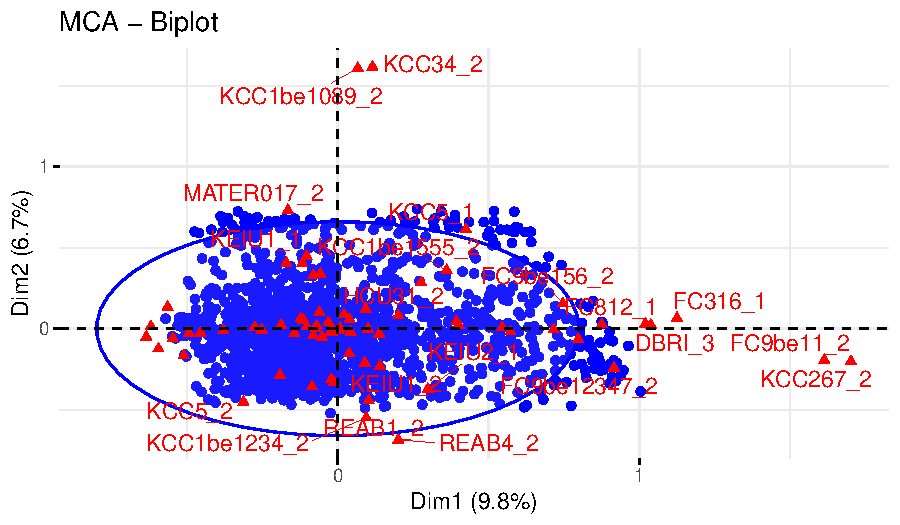
\includegraphics[width=\maxwidth]{figure/unnamed-chunk-12-1} 
\begin{kframe}\begin{verbatim}
## 
##  iter imp variable
##   1   1  LVLb  ICOS1  ICOS2  ICOS3  ICOS4  ICOS5  QPE1b  QPE2b  QPD1b  QPD2b  QPP1b  QPP2b  QME1b  QME2b  QME3b  CUI1b  CUI2b  CUI3b  CUI4b  CUI5b  ACTIVITE*  TMM1e1  TMM2e1  TMM3e1  TMMB1e1  TMMB2e1  TMMB3e1  TRM0e1  TRM1e1  TRM5e1  TRM7e1  TRP0e1  TRP1e1  TRP3e1  TRS1e1  TRS2e1  TRS3e1  TRS4e1  TRS5e1
##   1   2  LVLb  ICOS1  ICOS2  ICOS3  ICOS4  ICOS5  QPE1b  QPE2b  QPD1b  QPD2b  QPP1b  QPP2b  QME1b  QME2b  QME3b  CUI1b  CUI2b  CUI3b  CUI4b  CUI5b  ACTIVITE*  TMM1e1  TMM2e1  TMM3e1  TMMB1e1  TMMB2e1  TMMB3e1  TRM0e1  TRM1e1  TRM5e1  TRM7e1  TRP0e1  TRP1e1  TRP3e1  TRS1e1  TRS2e1  TRS3e1  TRS4e1  TRS5e1
##   1   3  LVLb  ICOS1  ICOS2  ICOS3  ICOS4  ICOS5  QPE1b  QPE2b  QPD1b  QPD2b  QPP1b  QPP2b  QME1b  QME2b  QME3b  CUI1b  CUI2b  CUI3b  CUI4b  CUI5b  ACTIVITE*  TMM1e1  TMM2e1  TMM3e1  TMMB1e1  TMMB2e1  TMMB3e1  TRM0e1  TRM1e1  TRM5e1  TRM7e1  TRP0e1  TRP1e1  TRP3e1  TRS1e1  TRS2e1  TRS3e1  TRS4e1  TRS5e1
##   1   4  LVLb  ICOS1  ICOS2  ICOS3  ICOS4  ICOS5  QPE1b  QPE2b  QPD1b  QPD2b  QPP1b  QPP2b  QME1b  QME2b  QME3b  CUI1b  CUI2b  CUI3b  CUI4b  CUI5b  ACTIVITE*  TMM1e1  TMM2e1  TMM3e1  TMMB1e1  TMMB2e1  TMMB3e1  TRM0e1  TRM1e1  TRM5e1  TRM7e1  TRP0e1  TRP1e1  TRP3e1  TRS1e1  TRS2e1  TRS3e1  TRS4e1  TRS5e1
##   1   5  LVLb  ICOS1  ICOS2  ICOS3  ICOS4  ICOS5  QPE1b  QPE2b  QPD1b  QPD2b  QPP1b  QPP2b  QME1b  QME2b  QME3b  CUI1b  CUI2b  CUI3b  CUI4b  CUI5b  ACTIVITE*  TMM1e1  TMM2e1  TMM3e1  TMMB1e1  TMMB2e1  TMMB3e1  TRM0e1  TRM1e1  TRM5e1  TRM7e1  TRP0e1  TRP1e1  TRP3e1  TRS1e1  TRS2e1  TRS3e1  TRS4e1  TRS5e1
##   2   1  LVLb  ICOS1  ICOS2  ICOS3  ICOS4  ICOS5  QPE1b  QPE2b  QPD1b  QPD2b  QPP1b  QPP2b  QME1b  QME2b  QME3b  CUI1b  CUI2b  CUI3b  CUI4b  CUI5b  ACTIVITE*  TMM1e1  TMM2e1  TMM3e1  TMMB1e1  TMMB2e1  TMMB3e1  TRM0e1  TRM1e1  TRM5e1  TRM7e1  TRP0e1  TRP1e1  TRP3e1  TRS1e1  TRS2e1  TRS3e1  TRS4e1  TRS5e1
##   2   2  LVLb  ICOS1  ICOS2  ICOS3  ICOS4  ICOS5  QPE1b  QPE2b  QPD1b  QPD2b  QPP1b  QPP2b  QME1b  QME2b  QME3b  CUI1b  CUI2b  CUI3b  CUI4b  CUI5b  ACTIVITE*  TMM1e1  TMM2e1  TMM3e1  TMMB1e1  TMMB2e1  TMMB3e1  TRM0e1  TRM1e1  TRM5e1  TRM7e1  TRP0e1  TRP1e1  TRP3e1  TRS1e1  TRS2e1  TRS3e1  TRS4e1  TRS5e1
##   2   3  LVLb  ICOS1  ICOS2  ICOS3  ICOS4  ICOS5  QPE1b  QPE2b  QPD1b  QPD2b  QPP1b  QPP2b  QME1b  QME2b  QME3b  CUI1b  CUI2b  CUI3b  CUI4b  CUI5b  ACTIVITE*  TMM1e1  TMM2e1  TMM3e1  TMMB1e1  TMMB2e1  TMMB3e1  TRM0e1  TRM1e1  TRM5e1  TRM7e1  TRP0e1  TRP1e1  TRP3e1  TRS1e1  TRS2e1  TRS3e1  TRS4e1  TRS5e1
##   2   4  LVLb  ICOS1  ICOS2  ICOS3  ICOS4  ICOS5  QPE1b  QPE2b  QPD1b  QPD2b  QPP1b  QPP2b  QME1b  QME2b  QME3b  CUI1b  CUI2b  CUI3b  CUI4b  CUI5b  ACTIVITE*  TMM1e1  TMM2e1  TMM3e1  TMMB1e1  TMMB2e1  TMMB3e1  TRM0e1  TRM1e1  TRM5e1  TRM7e1  TRP0e1  TRP1e1  TRP3e1  TRS1e1  TRS2e1  TRS3e1  TRS4e1  TRS5e1
##   2   5  LVLb  ICOS1  ICOS2  ICOS3  ICOS4  ICOS5  QPE1b  QPE2b  QPD1b  QPD2b  QPP1b  QPP2b  QME1b  QME2b  QME3b  CUI1b  CUI2b  CUI3b  CUI4b  CUI5b  ACTIVITE*  TMM1e1  TMM2e1  TMM3e1  TMMB1e1  TMMB2e1  TMMB3e1  TRM0e1  TRM1e1  TRM5e1  TRM7e1  TRP0e1  TRP1e1  TRP3e1  TRS1e1  TRS2e1  TRS3e1  TRS4e1  TRS5e1
##   3   1  LVLb  ICOS1  ICOS2  ICOS3  ICOS4  ICOS5  QPE1b  QPE2b  QPD1b  QPD2b  QPP1b  QPP2b  QME1b  QME2b  QME3b  CUI1b  CUI2b  CUI3b  CUI4b  CUI5b  ACTIVITE*  TMM1e1  TMM2e1  TMM3e1  TMMB1e1  TMMB2e1  TMMB3e1  TRM0e1  TRM1e1  TRM5e1  TRM7e1  TRP0e1  TRP1e1  TRP3e1  TRS1e1  TRS2e1  TRS3e1  TRS4e1  TRS5e1
##   3   2  LVLb  ICOS1  ICOS2  ICOS3  ICOS4  ICOS5  QPE1b  QPE2b  QPD1b  QPD2b  QPP1b  QPP2b  QME1b  QME2b  QME3b  CUI1b  CUI2b  CUI3b  CUI4b  CUI5b  ACTIVITE*  TMM1e1  TMM2e1  TMM3e1  TMMB1e1  TMMB2e1  TMMB3e1  TRM0e1  TRM1e1  TRM5e1  TRM7e1  TRP0e1  TRP1e1  TRP3e1  TRS1e1  TRS2e1  TRS3e1  TRS4e1  TRS5e1
##   3   3  LVLb  ICOS1  ICOS2  ICOS3  ICOS4  ICOS5  QPE1b  QPE2b  QPD1b  QPD2b  QPP1b  QPP2b  QME1b  QME2b  QME3b  CUI1b  CUI2b  CUI3b  CUI4b  CUI5b  ACTIVITE*  TMM1e1  TMM2e1  TMM3e1  TMMB1e1  TMMB2e1  TMMB3e1  TRM0e1  TRM1e1  TRM5e1  TRM7e1  TRP0e1  TRP1e1  TRP3e1  TRS1e1  TRS2e1  TRS3e1  TRS4e1  TRS5e1
##   3   4  LVLb  ICOS1  ICOS2  ICOS3  ICOS4  ICOS5  QPE1b  QPE2b  QPD1b  QPD2b  QPP1b  QPP2b  QME1b  QME2b  QME3b  CUI1b  CUI2b  CUI3b  CUI4b  CUI5b  ACTIVITE*  TMM1e1  TMM2e1  TMM3e1  TMMB1e1  TMMB2e1  TMMB3e1  TRM0e1  TRM1e1  TRM5e1  TRM7e1  TRP0e1  TRP1e1  TRP3e1  TRS1e1  TRS2e1  TRS3e1  TRS4e1  TRS5e1
##   3   5  LVLb  ICOS1  ICOS2  ICOS3  ICOS4  ICOS5  QPE1b  QPE2b  QPD1b  QPD2b  QPP1b  QPP2b  QME1b  QME2b  QME3b  CUI1b  CUI2b  CUI3b  CUI4b  CUI5b  ACTIVITE*  TMM1e1  TMM2e1  TMM3e1  TMMB1e1  TMMB2e1  TMMB3e1  TRM0e1  TRM1e1  TRM5e1  TRM7e1  TRP0e1  TRP1e1  TRP3e1  TRS1e1  TRS2e1  TRS3e1  TRS4e1  TRS5e1
##   4   1  LVLb  ICOS1  ICOS2  ICOS3  ICOS4  ICOS5  QPE1b  QPE2b  QPD1b  QPD2b  QPP1b  QPP2b  QME1b  QME2b  QME3b  CUI1b  CUI2b  CUI3b  CUI4b  CUI5b  ACTIVITE*  TMM1e1  TMM2e1  TMM3e1  TMMB1e1  TMMB2e1  TMMB3e1  TRM0e1  TRM1e1  TRM5e1  TRM7e1  TRP0e1  TRP1e1  TRP3e1  TRS1e1  TRS2e1  TRS3e1  TRS4e1  TRS5e1
##   4   2  LVLb  ICOS1  ICOS2  ICOS3  ICOS4  ICOS5  QPE1b  QPE2b  QPD1b  QPD2b  QPP1b  QPP2b  QME1b  QME2b  QME3b  CUI1b  CUI2b  CUI3b  CUI4b  CUI5b  ACTIVITE*  TMM1e1  TMM2e1  TMM3e1  TMMB1e1  TMMB2e1  TMMB3e1  TRM0e1  TRM1e1  TRM5e1  TRM7e1  TRP0e1  TRP1e1  TRP3e1  TRS1e1  TRS2e1  TRS3e1  TRS4e1  TRS5e1
##   4   3  LVLb  ICOS1  ICOS2  ICOS3  ICOS4  ICOS5  QPE1b  QPE2b  QPD1b  QPD2b  QPP1b  QPP2b  QME1b  QME2b  QME3b  CUI1b  CUI2b  CUI3b  CUI4b  CUI5b  ACTIVITE*  TMM1e1  TMM2e1  TMM3e1  TMMB1e1  TMMB2e1  TMMB3e1  TRM0e1  TRM1e1  TRM5e1  TRM7e1  TRP0e1  TRP1e1  TRP3e1  TRS1e1  TRS2e1  TRS3e1  TRS4e1  TRS5e1
##   4   4  LVLb  ICOS1  ICOS2  ICOS3  ICOS4  ICOS5  QPE1b  QPE2b  QPD1b  QPD2b  QPP1b  QPP2b  QME1b  QME2b  QME3b  CUI1b  CUI2b  CUI3b  CUI4b  CUI5b  ACTIVITE*  TMM1e1  TMM2e1  TMM3e1  TMMB1e1  TMMB2e1  TMMB3e1  TRM0e1  TRM1e1  TRM5e1  TRM7e1  TRP0e1  TRP1e1  TRP3e1  TRS1e1  TRS2e1  TRS3e1  TRS4e1  TRS5e1
##   4   5  LVLb  ICOS1  ICOS2  ICOS3  ICOS4  ICOS5  QPE1b  QPE2b  QPD1b  QPD2b  QPP1b  QPP2b  QME1b  QME2b  QME3b  CUI1b  CUI2b  CUI3b  CUI4b  CUI5b  ACTIVITE*  TMM1e1  TMM2e1  TMM3e1  TMMB1e1  TMMB2e1  TMMB3e1  TRM0e1  TRM1e1  TRM5e1  TRM7e1  TRP0e1  TRP1e1  TRP3e1  TRS1e1  TRS2e1  TRS3e1  TRS4e1  TRS5e1
##   5   1  LVLb  ICOS1  ICOS2  ICOS3  ICOS4  ICOS5  QPE1b  QPE2b  QPD1b  QPD2b  QPP1b  QPP2b  QME1b  QME2b  QME3b  CUI1b  CUI2b  CUI3b  CUI4b  CUI5b  ACTIVITE*  TMM1e1  TMM2e1  TMM3e1  TMMB1e1  TMMB2e1  TMMB3e1  TRM0e1  TRM1e1  TRM5e1  TRM7e1  TRP0e1  TRP1e1  TRP3e1  TRS1e1  TRS2e1  TRS3e1  TRS4e1  TRS5e1
##   5   2  LVLb  ICOS1  ICOS2  ICOS3  ICOS4  ICOS5  QPE1b  QPE2b  QPD1b  QPD2b  QPP1b  QPP2b  QME1b  QME2b  QME3b  CUI1b  CUI2b  CUI3b  CUI4b  CUI5b  ACTIVITE*  TMM1e1  TMM2e1  TMM3e1  TMMB1e1  TMMB2e1  TMMB3e1  TRM0e1  TRM1e1  TRM5e1  TRM7e1  TRP0e1  TRP1e1  TRP3e1  TRS1e1  TRS2e1  TRS3e1  TRS4e1  TRS5e1
##   5   3  LVLb  ICOS1  ICOS2  ICOS3  ICOS4  ICOS5  QPE1b  QPE2b  QPD1b  QPD2b  QPP1b  QPP2b  QME1b  QME2b  QME3b  CUI1b  CUI2b  CUI3b  CUI4b  CUI5b  ACTIVITE*  TMM1e1  TMM2e1  TMM3e1  TMMB1e1  TMMB2e1  TMMB3e1  TRM0e1  TRM1e1  TRM5e1  TRM7e1  TRP0e1  TRP1e1  TRP3e1  TRS1e1  TRS2e1  TRS3e1  TRS4e1  TRS5e1
##   5   4  LVLb  ICOS1  ICOS2  ICOS3  ICOS4  ICOS5  QPE1b  QPE2b  QPD1b  QPD2b  QPP1b  QPP2b  QME1b  QME2b  QME3b  CUI1b  CUI2b  CUI3b  CUI4b  CUI5b  ACTIVITE*  TMM1e1  TMM2e1  TMM3e1  TMMB1e1  TMMB2e1  TMMB3e1  TRM0e1  TRM1e1  TRM5e1  TRM7e1  TRP0e1  TRP1e1  TRP3e1  TRS1e1  TRS2e1  TRS3e1  TRS4e1  TRS5e1
##   5   5  LVLb  ICOS1  ICOS2  ICOS3  ICOS4  ICOS5  QPE1b  QPE2b  QPD1b  QPD2b  QPP1b  QPP2b  QME1b  QME2b  QME3b  CUI1b  CUI2b  CUI3b  CUI4b  CUI5b  ACTIVITE*  TMM1e1  TMM2e1  TMM3e1  TMMB1e1  TMMB2e1  TMMB3e1  TRM0e1  TRM1e1  TRM5e1  TRM7e1  TRP0e1  TRP1e1  TRP3e1  TRS1e1  TRS2e1  TRS3e1  TRS4e1  TRS5e1
\end{verbatim}
\end{kframe}
\end{knitrout}

\begin{knitrout}
\definecolor{shadecolor}{rgb}{1, 1, 1}\color{fgcolor}
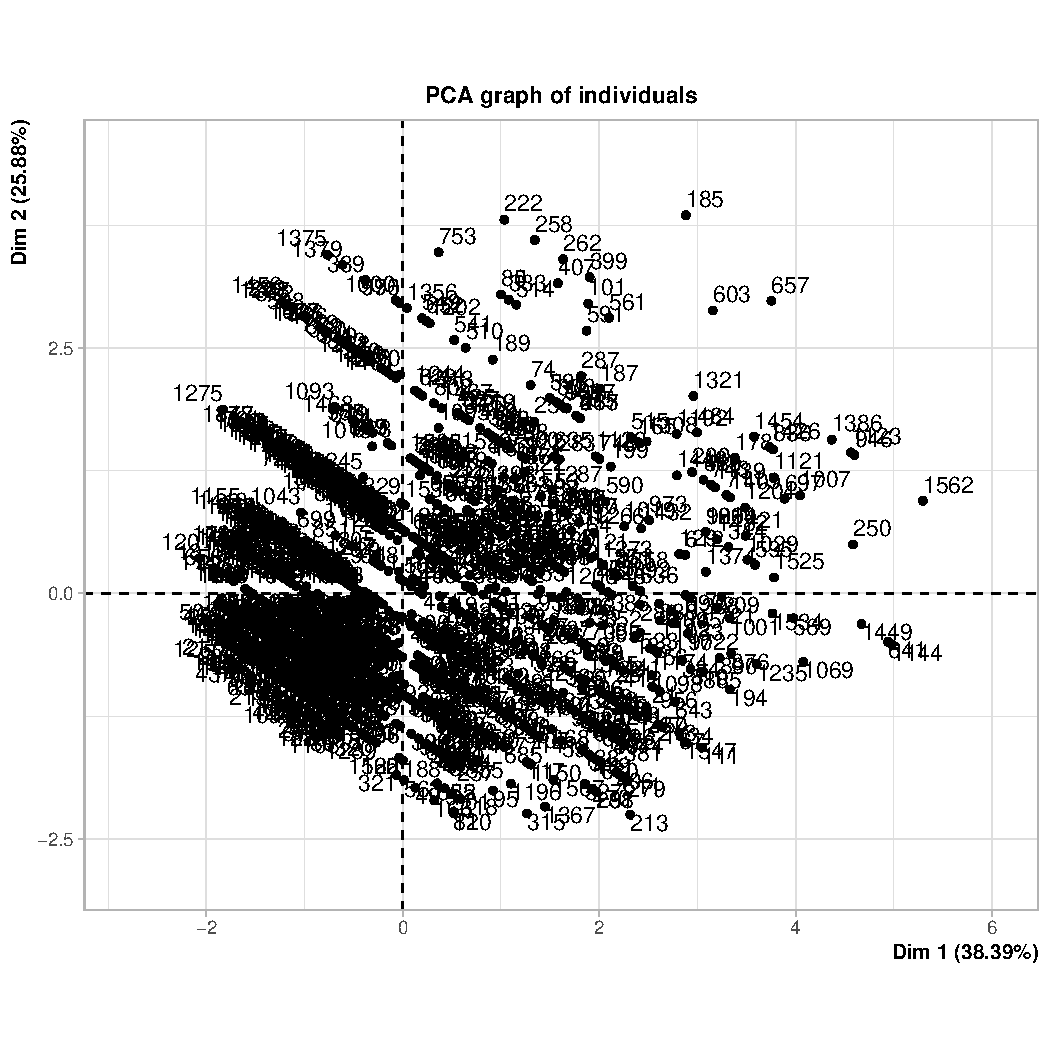
\includegraphics[width=\maxwidth]{figure/acp-1} 

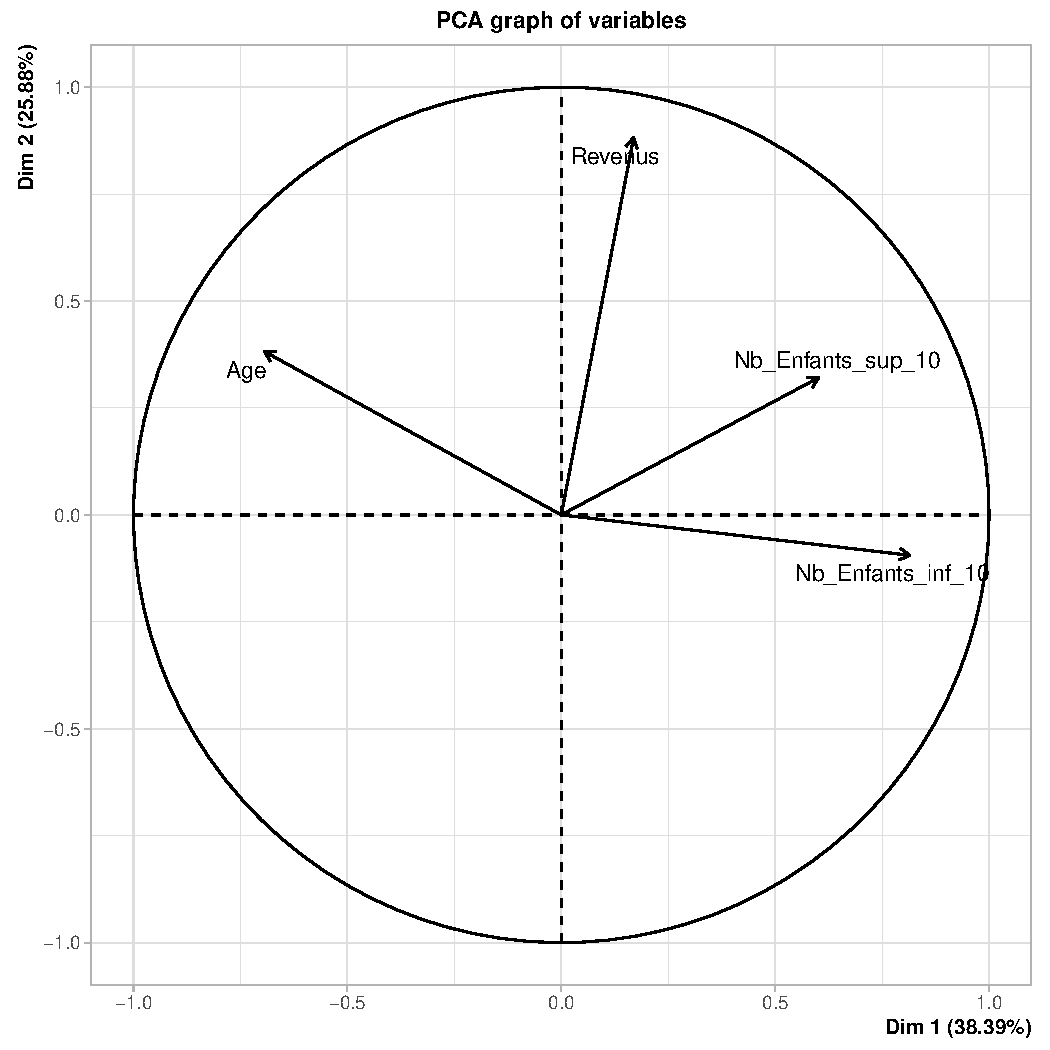
\includegraphics[width=\maxwidth]{figure/acp-2} 
\end{knitrout}

\begin{figure}[H]
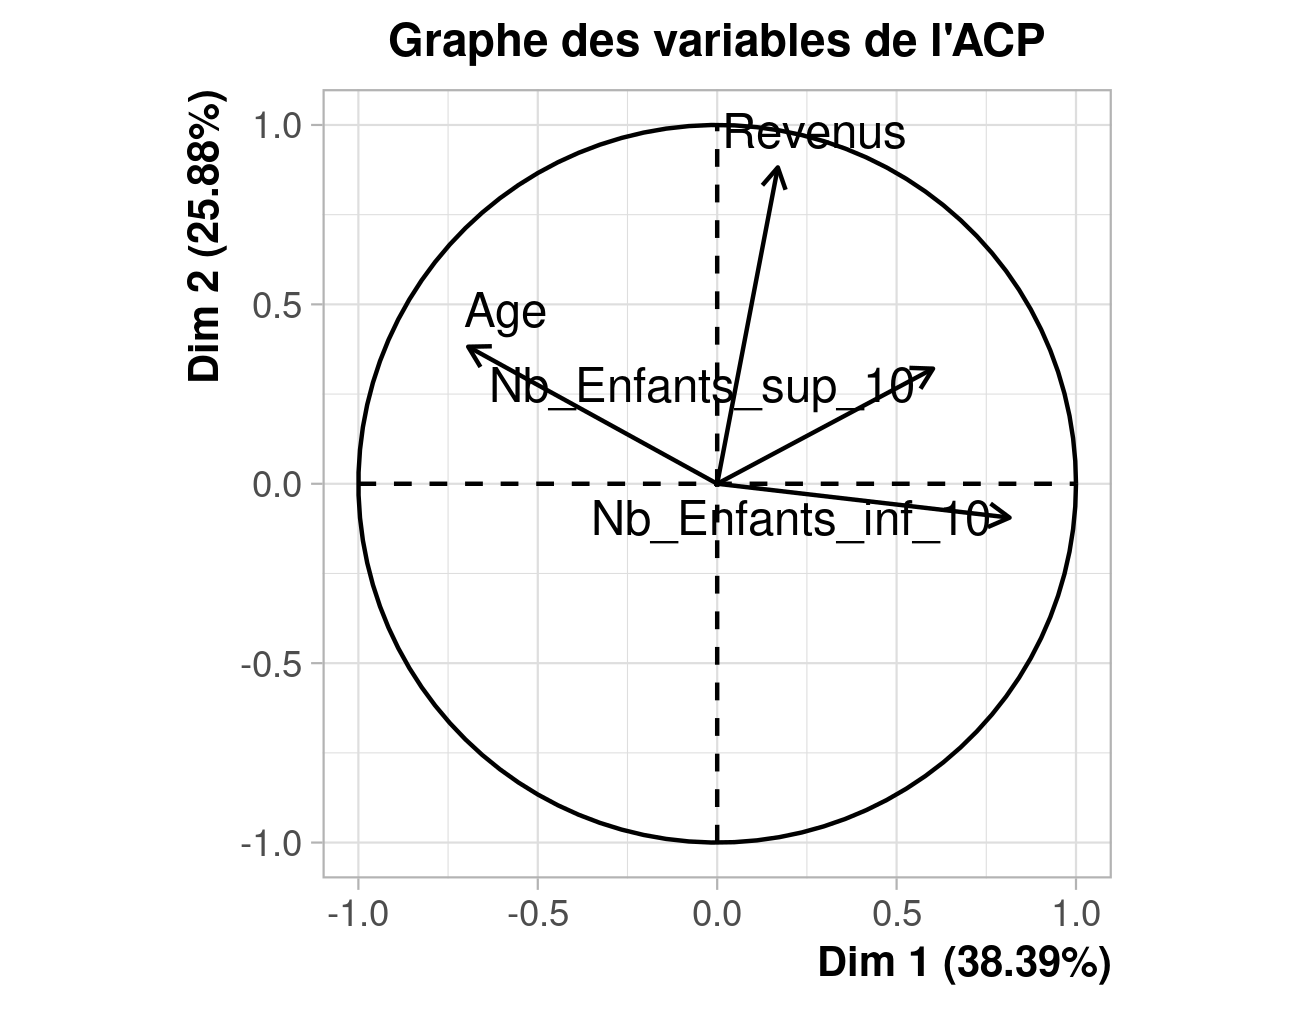
\includegraphics[]{Images/graphVar.png}
\end{figure}

Les 2 premiers axes de l’ ACP  expriment 64.27\% de l’inertie totale du jeu de données ; cela signifie que 64.27\% de la variabilité totale du nuage est représentée dans ce plan. C’est un pourcentage assez important, et le premier plan représente donc convenablement la variabilité contenue dans une grande part du jeu de données constitué des variables numériques . Cette valeur est supérieure à la valeur référence de 52.76\%, la variabilité expliquée par ce plan est donc significative (cette intertie de référence est le quantile 0.95-quantile de la distribution des pourcentages d’inertie obtenue en simulant 2779 jeux de données aléatoires de dimensions comparables sur la base d’une distribution normale).

Du fait de ces observations, il serait tout de même probablement préférable de considérer également dans l’analyse les dimensions supérieures ou égales à la troisième.
\begin{knitrout}
\definecolor{shadecolor}{rgb}{1, 1, 1}\color{fgcolor}
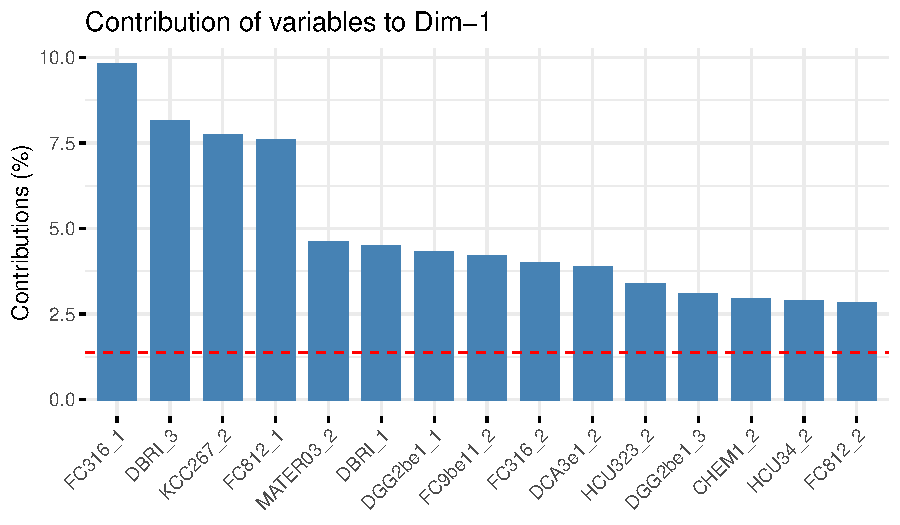
\includegraphics[width=\maxwidth]{figure/unnamed-chunk-13-1} 

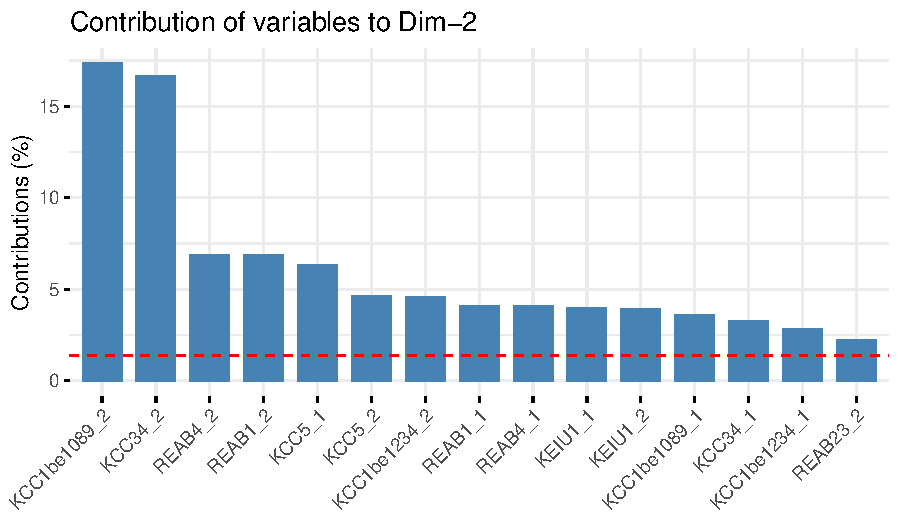
\includegraphics[width=\maxwidth]{figure/unnamed-chunk-13-2} 

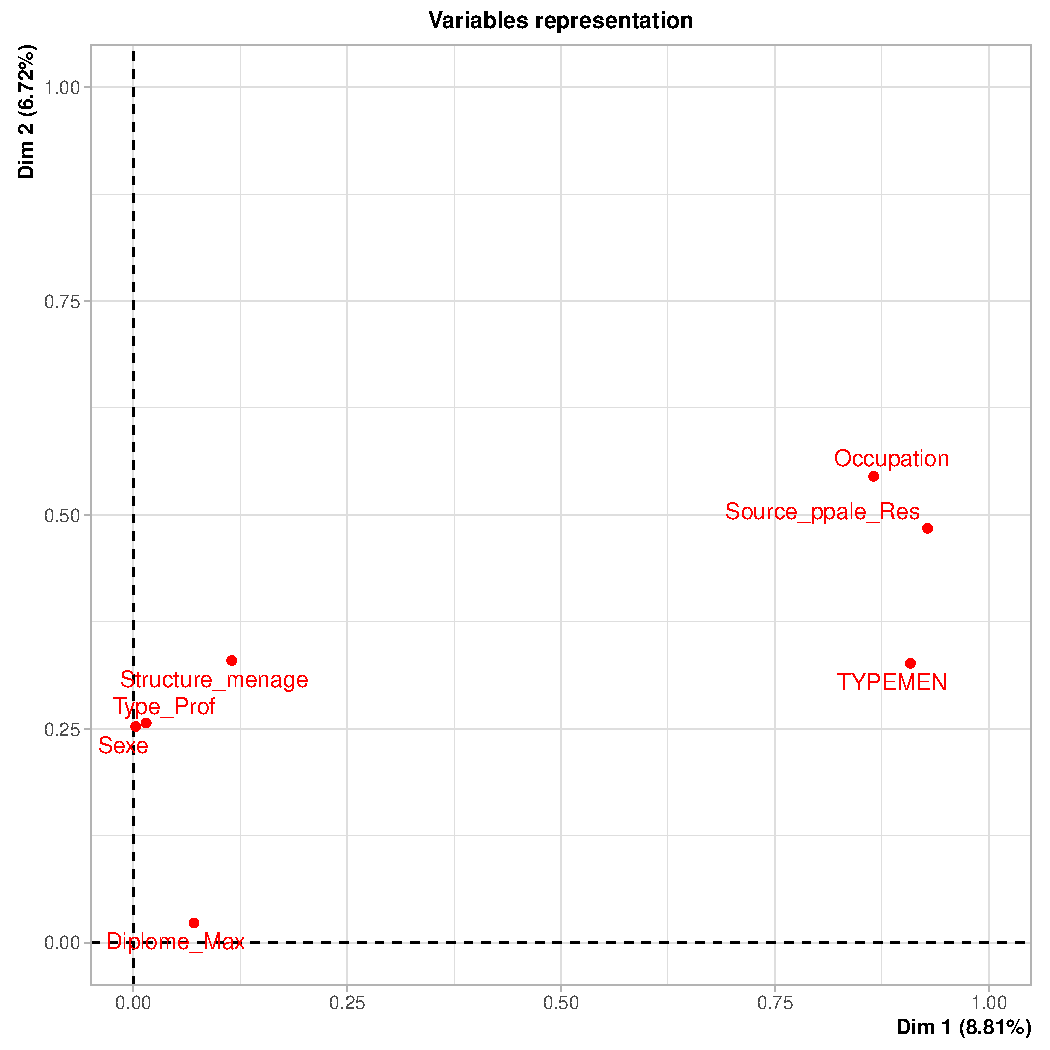
\includegraphics[width=\maxwidth]{figure/unnamed-chunk-13-3} 

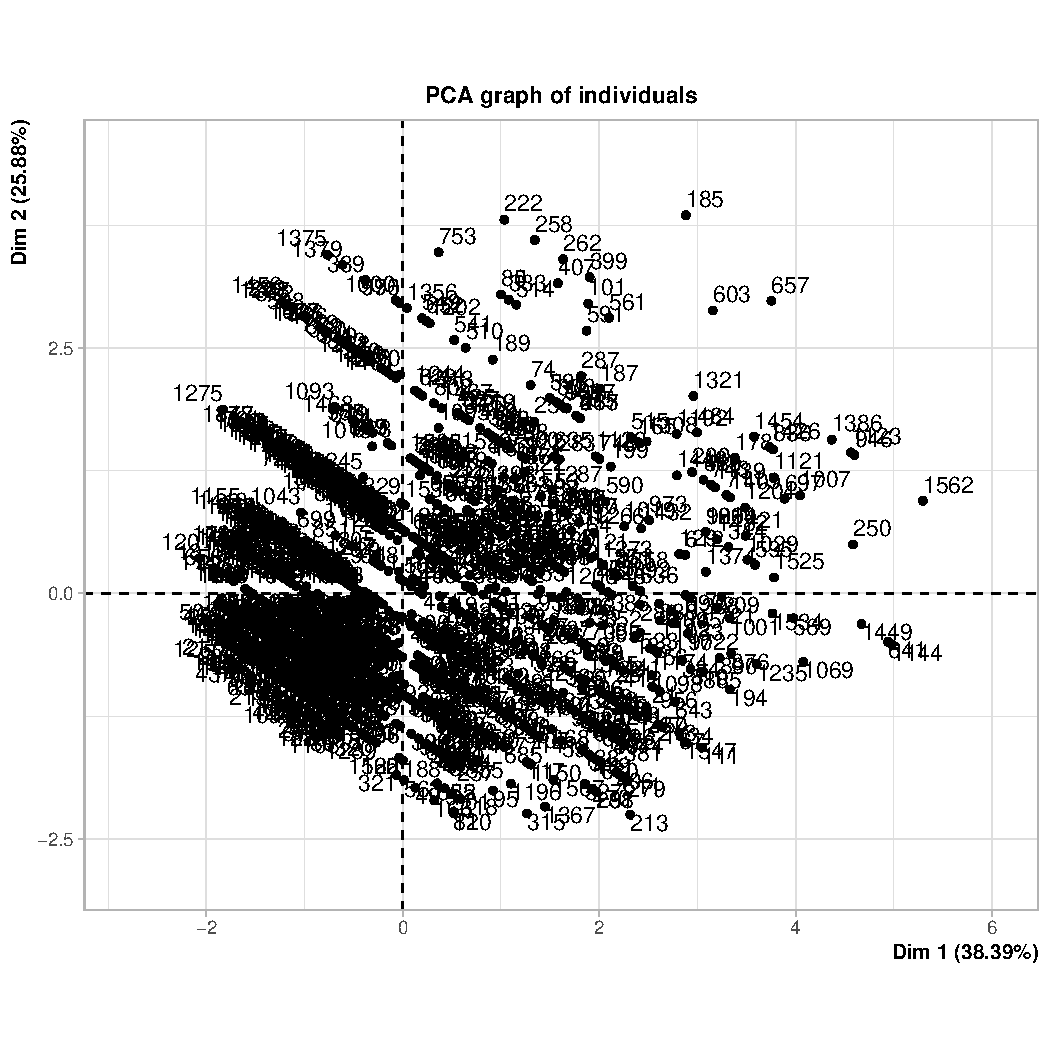
\includegraphics[width=\maxwidth]{figure/unnamed-chunk-13-4} 

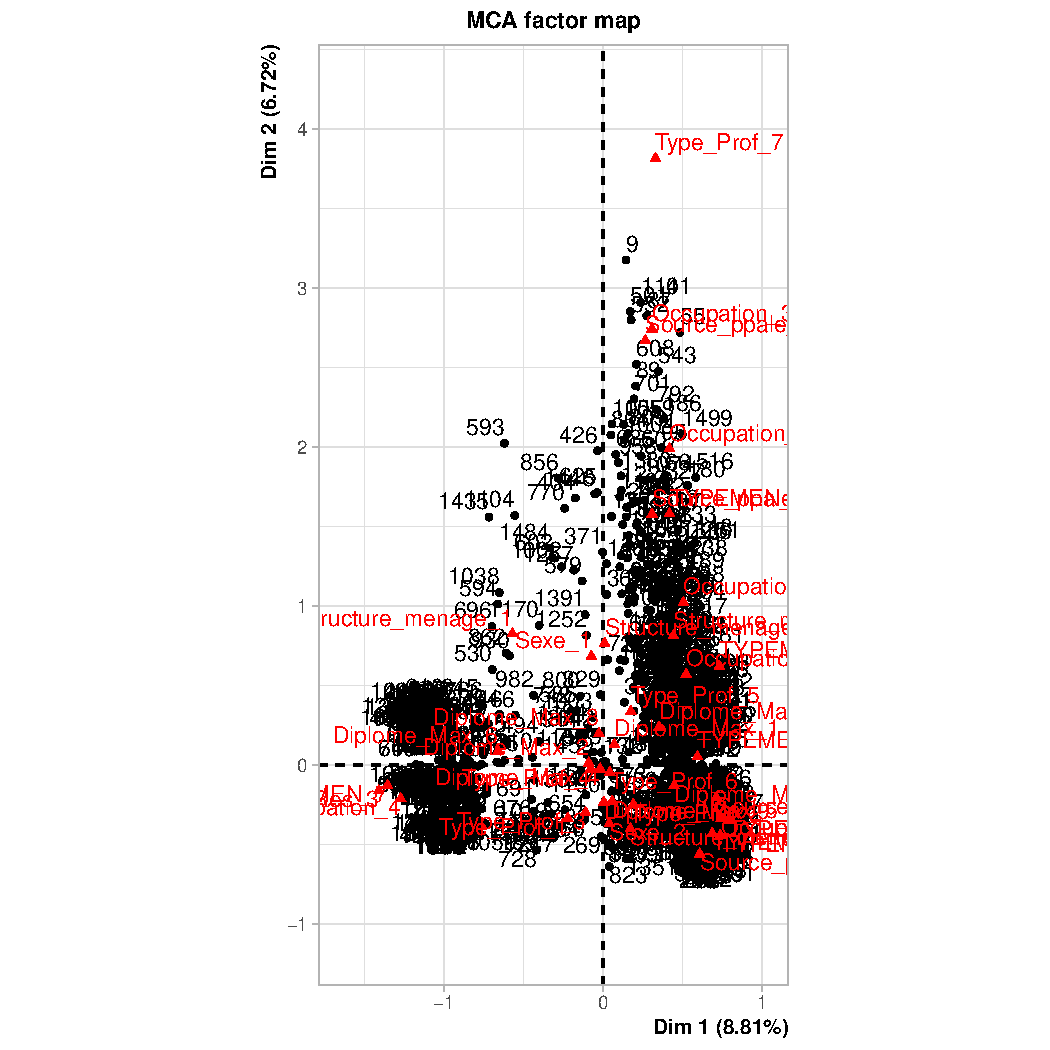
\includegraphics[width=\maxwidth]{figure/unnamed-chunk-13-5} 
\end{knitrout}


\end{document}

